% Options for packages loaded elsewhere
\PassOptionsToPackage{unicode}{hyperref}
\PassOptionsToPackage{hyphens}{url}
%
\documentclass[
]{book}
\usepackage{amsmath,amssymb}
\usepackage{lmodern}
\usepackage{iftex}
\ifPDFTeX
  \usepackage[T1]{fontenc}
  \usepackage[utf8]{inputenc}
  \usepackage{textcomp} % provide euro and other symbols
\else % if luatex or xetex
  \usepackage{unicode-math}
  \defaultfontfeatures{Scale=MatchLowercase}
  \defaultfontfeatures[\rmfamily]{Ligatures=TeX,Scale=1}
\fi
% Use upquote if available, for straight quotes in verbatim environments
\IfFileExists{upquote.sty}{\usepackage{upquote}}{}
\IfFileExists{microtype.sty}{% use microtype if available
  \usepackage[]{microtype}
  \UseMicrotypeSet[protrusion]{basicmath} % disable protrusion for tt fonts
}{}
\makeatletter
\@ifundefined{KOMAClassName}{% if non-KOMA class
  \IfFileExists{parskip.sty}{%
    \usepackage{parskip}
  }{% else
    \setlength{\parindent}{0pt}
    \setlength{\parskip}{6pt plus 2pt minus 1pt}}
}{% if KOMA class
  \KOMAoptions{parskip=half}}
\makeatother
\usepackage{xcolor}
\usepackage{color}
\usepackage{fancyvrb}
\newcommand{\VerbBar}{|}
\newcommand{\VERB}{\Verb[commandchars=\\\{\}]}
\DefineVerbatimEnvironment{Highlighting}{Verbatim}{commandchars=\\\{\}}
% Add ',fontsize=\small' for more characters per line
\usepackage{framed}
\definecolor{shadecolor}{RGB}{248,248,248}
\newenvironment{Shaded}{\begin{snugshade}}{\end{snugshade}}
\newcommand{\AlertTok}[1]{\textcolor[rgb]{0.94,0.16,0.16}{#1}}
\newcommand{\AnnotationTok}[1]{\textcolor[rgb]{0.56,0.35,0.01}{\textbf{\textit{#1}}}}
\newcommand{\AttributeTok}[1]{\textcolor[rgb]{0.77,0.63,0.00}{#1}}
\newcommand{\BaseNTok}[1]{\textcolor[rgb]{0.00,0.00,0.81}{#1}}
\newcommand{\BuiltInTok}[1]{#1}
\newcommand{\CharTok}[1]{\textcolor[rgb]{0.31,0.60,0.02}{#1}}
\newcommand{\CommentTok}[1]{\textcolor[rgb]{0.56,0.35,0.01}{\textit{#1}}}
\newcommand{\CommentVarTok}[1]{\textcolor[rgb]{0.56,0.35,0.01}{\textbf{\textit{#1}}}}
\newcommand{\ConstantTok}[1]{\textcolor[rgb]{0.00,0.00,0.00}{#1}}
\newcommand{\ControlFlowTok}[1]{\textcolor[rgb]{0.13,0.29,0.53}{\textbf{#1}}}
\newcommand{\DataTypeTok}[1]{\textcolor[rgb]{0.13,0.29,0.53}{#1}}
\newcommand{\DecValTok}[1]{\textcolor[rgb]{0.00,0.00,0.81}{#1}}
\newcommand{\DocumentationTok}[1]{\textcolor[rgb]{0.56,0.35,0.01}{\textbf{\textit{#1}}}}
\newcommand{\ErrorTok}[1]{\textcolor[rgb]{0.64,0.00,0.00}{\textbf{#1}}}
\newcommand{\ExtensionTok}[1]{#1}
\newcommand{\FloatTok}[1]{\textcolor[rgb]{0.00,0.00,0.81}{#1}}
\newcommand{\FunctionTok}[1]{\textcolor[rgb]{0.00,0.00,0.00}{#1}}
\newcommand{\ImportTok}[1]{#1}
\newcommand{\InformationTok}[1]{\textcolor[rgb]{0.56,0.35,0.01}{\textbf{\textit{#1}}}}
\newcommand{\KeywordTok}[1]{\textcolor[rgb]{0.13,0.29,0.53}{\textbf{#1}}}
\newcommand{\NormalTok}[1]{#1}
\newcommand{\OperatorTok}[1]{\textcolor[rgb]{0.81,0.36,0.00}{\textbf{#1}}}
\newcommand{\OtherTok}[1]{\textcolor[rgb]{0.56,0.35,0.01}{#1}}
\newcommand{\PreprocessorTok}[1]{\textcolor[rgb]{0.56,0.35,0.01}{\textit{#1}}}
\newcommand{\RegionMarkerTok}[1]{#1}
\newcommand{\SpecialCharTok}[1]{\textcolor[rgb]{0.00,0.00,0.00}{#1}}
\newcommand{\SpecialStringTok}[1]{\textcolor[rgb]{0.31,0.60,0.02}{#1}}
\newcommand{\StringTok}[1]{\textcolor[rgb]{0.31,0.60,0.02}{#1}}
\newcommand{\VariableTok}[1]{\textcolor[rgb]{0.00,0.00,0.00}{#1}}
\newcommand{\VerbatimStringTok}[1]{\textcolor[rgb]{0.31,0.60,0.02}{#1}}
\newcommand{\WarningTok}[1]{\textcolor[rgb]{0.56,0.35,0.01}{\textbf{\textit{#1}}}}
\usepackage{longtable,booktabs,array}
\usepackage{calc} % for calculating minipage widths
% Correct order of tables after \paragraph or \subparagraph
\usepackage{etoolbox}
\makeatletter
\patchcmd\longtable{\par}{\if@noskipsec\mbox{}\fi\par}{}{}
\makeatother
% Allow footnotes in longtable head/foot
\IfFileExists{footnotehyper.sty}{\usepackage{footnotehyper}}{\usepackage{footnote}}
\makesavenoteenv{longtable}
\usepackage{graphicx}
\makeatletter
\def\maxwidth{\ifdim\Gin@nat@width>\linewidth\linewidth\else\Gin@nat@width\fi}
\def\maxheight{\ifdim\Gin@nat@height>\textheight\textheight\else\Gin@nat@height\fi}
\makeatother
% Scale images if necessary, so that they will not overflow the page
% margins by default, and it is still possible to overwrite the defaults
% using explicit options in \includegraphics[width, height, ...]{}
\setkeys{Gin}{width=\maxwidth,height=\maxheight,keepaspectratio}
% Set default figure placement to htbp
\makeatletter
\def\fps@figure{htbp}
\makeatother
\usepackage[normalem]{ulem}
\setlength{\emergencystretch}{3em} % prevent overfull lines
\providecommand{\tightlist}{%
  \setlength{\itemsep}{0pt}\setlength{\parskip}{0pt}}
\setcounter{secnumdepth}{5}
\usepackage{booktabs}
\ifLuaTeX
  \usepackage{selnolig}  % disable illegal ligatures
\fi
\usepackage[]{natbib}
\bibliographystyle{apalike}
\IfFileExists{bookmark.sty}{\usepackage{bookmark}}{\usepackage{hyperref}}
\IfFileExists{xurl.sty}{\usepackage{xurl}}{} % add URL line breaks if available
\urlstyle{same} % disable monospaced font for URLs
\hypersetup{
  pdftitle={初級統計学},
  pdfauthor={TI},
  hidelinks,
  pdfcreator={LaTeX via pandoc}}

\title{初級統計学}
\author{TI}
\date{2023-03-08}

\usepackage{amsthm}
\newtheorem{theorem}{Theorem}[chapter]
\newtheorem{lemma}{Lemma}[chapter]
\newtheorem{corollary}{Corollary}[chapter]
\newtheorem{proposition}{Proposition}[chapter]
\newtheorem{conjecture}{Conjecture}[chapter]
\theoremstyle{definition}
\newtheorem{definition}{Definition}[chapter]
\theoremstyle{definition}
\newtheorem{example}{Example}[chapter]
\theoremstyle{definition}
\newtheorem{exercise}{Exercise}[chapter]
\theoremstyle{definition}
\newtheorem{hypothesis}{Hypothesis}[chapter]
\theoremstyle{remark}
\newtheorem*{remark}{Remark}
\newtheorem*{solution}{Solution}
\begin{document}
\maketitle

{
\setcounter{tocdepth}{1}
\tableofcontents
}
\hypertarget{ux7de8ux96c6ux7528}{%
\chapter*{編集用}\label{ux7de8ux96c6ux7528}}
\addcontentsline{toc}{chapter}{編集用}

\url{https://bookdown.org/yihui/rmarkdown-cookbook/}

Qiita マークダウン記法 一覧表・チートシート
\url{https://qiita.com/kamorits/items/6f342da395ad57468ae3}

This is a \emph{sample} book written in \textbf{Markdown}. You can use anything that Pandoc's Markdown supports; for example, a math equation \(a^2 + b^2 = c^2\).

\hypertarget{usage}{%
\section{Usage}\label{usage}}

Each \textbf{bookdown} chapter is an .Rmd file, and each .Rmd file can contain one (and only one) chapter. A chapter \emph{must} start with a first-level heading: \texttt{\#\ A\ good\ chapter}, and can contain one (and only one) first-level heading.

Use second-level and higher headings within chapters like: \texttt{\#\#\ A\ short\ section} or \texttt{\#\#\#\ An\ even\ shorter\ section}.

The \texttt{index.Rmd} file is required, and is also your first book chapter. It will be the homepage when you render the book.

\hypertarget{render-book}{%
\section{Render book}\label{render-book}}

You can render the HTML version of this example book without changing anything:

\begin{enumerate}
\def\labelenumi{\arabic{enumi}.}
\item
  Find the \textbf{Build} pane in the RStudio IDE, and
\item
  Click on \textbf{Build Book}, then select your output format, or select ``All formats'' if you'd like to use multiple formats from the same book source files.
\end{enumerate}

Or build the book from the R console:

\begin{Shaded}
\begin{Highlighting}[]
\NormalTok{bookdown}\SpecialCharTok{::}\FunctionTok{render\_book}\NormalTok{()}
\end{Highlighting}
\end{Shaded}

To render this example to PDF as a \texttt{bookdown::pdf\_book}, you'll need to install XeLaTeX. You are recommended to install TinyTeX (which includes XeLaTeX): \url{https://yihui.org/tinytex/}.

\hypertarget{preview-book}{%
\section{Preview book}\label{preview-book}}

As you work, you may start a local server to live preview this HTML book. This preview will update as you edit the book when you save individual .Rmd files. You can start the server in a work session by using the RStudio add-in ``Preview book'', or from the R console:

\begin{Shaded}
\begin{Highlighting}[]
\NormalTok{bookdown}\SpecialCharTok{::}\FunctionTok{serve\_book}\NormalTok{()}
\end{Highlighting}
\end{Shaded}

\hypertarget{part-ux7b2cuxff11ux90e8}{%
\chapter{(PART*) 第1部}\label{part-ux7b2cuxff11ux90e8}}

\hypertarget{ux7d71ux8a08ux3068ux4ebaux9593ux751fux6d3b}{%
\chapter{統計と人間生活}\label{ux7d71ux8a08ux3068ux4ebaux9593ux751fux6d3b}}

日常生活では\textbf{統計的な考え方}がさまざまな場面で利用されている

\begin{quote}
例1:統計がないとスポーツ観戦がつまらなくなる
野球では,過去の対戦成績(○勝△敗),打撃成績(○割○分○厘),投手成績(防御率)のような\textbf{統計}が利用される

\[
\text{打率}=\frac{\text{安打}}{\text{打数}} \qquad\qquad
\text{防御率}=\frac{\text{自責点}}{\text{投球回}} \times 9
\]
\end{quote}

これらの\textbf{統計}が存在しなければ:

\begin{itemize}
\tightlist
\item
  登場した打者にどれくらいの安打が期待できるのかわからない
\item
  投手にどれくらいの健闘が期待できるのかわからない
\end{itemize}

\begin{quote}
例2:統計がないと今日の天気を比べられない
天気予報で気象予報士が「きょうは4月中旬にしては異常に暖かかった」あるいは「きょうは6月上旬の陽気であった」と表現することがある。
\end{quote}

\begin{itemize}
\tightlist
\item
  「異常」な状態を定義するには,「平常」な状態の定義が必要
\item
  ではどのように「平常」な状態を定義できるだろうか?
\item
  「平常」な気温は,過去何十年にもわたって観測した4月中旬の気温を平均してもとめた\underline{平均気温}という統計数字
\item
  「異常」な暖かさとは「平常」な気温の値があってはじめて判断できる
\item
  疑問:平均気温よりもどれくらい離れていると「異常」と言えるだろうか?
\end{itemize}

\begin{quote}
例3:統計がなければ「当選確実」かどうかはすぐにわからない
選挙速報で,数パーセントしか開票していないのに「当選確実」と報道できるのはなぜか?
\end{quote}

\begin{itemize}
\tightlist
\item
  選挙前の支持者,投票意向などの統計的調査などから得た情報をもとに``推定'\,'
\item
  \textbf{一部分の開票結果}から\textbf{全体の傾向}を推しはかる``統計的推論'\,'とよばれる分析の応用例
\end{itemize}

\begin{quote}
例4:企業経営に統計は不可欠
多くの製造業者は,注文を受けてから製品を製造する\textbf{受注生産}ではなく,どれくらい売れそうかという見込みをたてて製品を製造する\textbf{見込生産}を行っている
\end{quote}

\begin{itemize}
\tightlist
\item
  生産量が多すぎれば\textbf{在庫}を抱えてしまうし,少なすぎたりすると社会的に混乱を生じさせてしまう

  \begin{itemize}
  \tightlist
  \item
    例:食品メーカーのある炭酸飲料が「予想を上回る注文があったため販売2日目で当面出荷停止」
  \item
    サントリーのオランジーナ 2015/4/2
  \end{itemize}
\item
  人口総数,男女別構成・年齢別構成等の統計をもとに需要予測を行い,生産量の計画をたてる
\item
  消費者の消費習慣や購買習慣を,企業みずから,あるいは専門の調査機関に依頼して\textbf{市場調査}する
\end{itemize}

\begin{quote}
例5:経済政策の決定にも統計は不可欠
政府は所得税を減税することで消費を増加させ,公共投資を増やすことによって景気を刺激しようとする。政策を決定する際には,各種の経済統計(家計調査,設備投資計画調査など)が示す経済状態に細心の注意を払うと同時に,各種税率,公共投資額,金利,マネーストック等の経済政策にかかわる変数と経済の状態を示す各種変数との関係が利用されている
\end{quote}

\begin{itemize}
\tightlist
\item
  GDP,物価指数,金利,株価,失業率,為替レートなどのマクロ経済データを使って作成した計量経済学的モデルは,政府の経済政策の決定に不可欠なツールのひとつ
\end{itemize}

\begin{quote}
内閣府の経済社会総合研究所の分析(2015)

\begin{itemize}
\tightlist
\item
  消費税率1\%引上げで1年後の実質GDPは0.24\%減少
\item
  短期金利1\%引上げで1年後の実質GDPは0.32\%減少
\item
  内閣府経済社会総合研究所「短期日本経済マクロ計量モデル(2015年版)の構造と乗数分析」
  \%(\url{http://www.esri.go.jp/jp/archive/e/_dis/e/_dis314/e/_dis314.pdf})
\end{itemize}
\end{quote}

\begin{quote}
例6:アパート・マンションを選ぶときにも統計が使える
この部屋の家賃は平均よりも高いのか、それとも安いのか?
\end{quote}

\begin{figure}
\centering
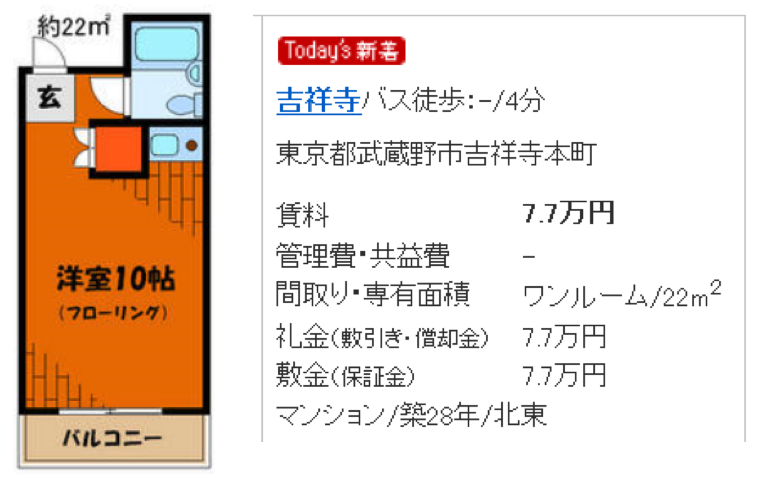
\includegraphics[width=0.5\textwidth,height=\textheight]{images/lec01/fig_kichi_1room_example.png}
\caption{image of histogram}
\end{figure}

\hypertarget{ux7d71ux8a08ux3068ux306f}{%
\section{統計とは}\label{ux7d71ux8a08ux3068ux306f}}

\begin{quote}
統計とは
統計とは,ある特定の集団について,それを構成するものの特定の性質に注目して観察し,その集団全体の特徴を数量的に表現しようとするもの
\end{quote}

\begin{itemize}
\tightlist
\item
  \textbf{記述統計}:複数の者,あるいは複数の時点で示した数字を集約整理し,その集団全体の\textbf{特徴を示そうとする}もの
\item
  \textbf{推測統計}:一部から全体の\textbf{特徴を推測・予測する}こと
\end{itemize}

\begin{quote}
質問
先述の例を分類してみましょう

\begin{longtable}[]{@{}ccc@{}}
\toprule()
& テーマ & 種類 \\
\midrule()
\endhead
例1 & スポーツ観戦 & データの要約(平均的傾向),記述 \\
例2 & 異常な天気 & データの要約(ちらばり具合) \\
例3 & 選挙速報 & 予測,推定 \\
例4 & 見込み生産 & 予測,推定 \\
例5 & 経済政策 & 記述,推定 \\
\bottomrule()
\end{longtable}
\end{quote}

\hypertarget{ux30c7ux30fcux30bfux306eux5c3aux5ea6ux306aux3069}{%
\chapter{データの尺度など}\label{ux30c7ux30fcux30bfux306eux5c3aux5ea6ux306aux3069}}

\hypertarget{ux30c7ux30fcux30bfux306eux5c3aux5ea6}{%
\section{データの尺度}\label{ux30c7ux30fcux30bfux306eux5c3aux5ea6}}

\begin{itemize}
\tightlist
\item
  データを作りあげている値にはさまざまな種類がある
\end{itemize}

\begin{quote}
例:ある大学の学生の成績・個人情報にかかわるデータ
\end{quote}

\begin{longtable}[]{@{}lllllll@{}}
\toprule()
学生ID & 学年 & 英語 & ミクロ & \(\cdots\) & GPA & 通学時間(分) \\
\midrule()
\endhead
155001 & 3 & S & A & \(\cdots\) & 3.67 & 45 \\
155002 & 3 & C & B & \(\cdots\) & 1.73 & 90 \\
: & : & : & : & & : & : \\
名義 & 順序 & 順序 & 順序 & & 間隔 & 比例 \\
\bottomrule()
\end{longtable}

\[
\text{変数}
\begin{cases}
\text{質的変数}
\begin{cases}
\text{名義尺度} & \text{同じ値かどうかを区別} \\
\text{順序尺度} & \text{値の大小関係のみ} \\
\end{cases} \\
\text{量的変数}
\begin{cases}
\text{間隔尺度} & \text{数値の間隔のみに意味がある} \\
\text{比例尺度} & \text{数値の間隔と比率に意味がある} \\
\end{cases}
\end{cases}
\]

\hypertarget{ux30c7ux30fcux30bfux306eux8868ux8a18ux65b9ux6cd5}{%
\section{データの表記方法}\label{ux30c7ux30fcux30bfux306eux8868ux8a18ux65b9ux6cd5}}

\hypertarget{ux5e79ux8449ux56f3stem-and-leaf}{%
\section{幹葉図(Stem-and-Leaf)}\label{ux5e79ux8449ux56f3stem-and-leaf}}

\begin{quote}
問題:学生の成績データ(幹葉図)
次の学生50人の成績データ(点数)で\textbf{幹葉図}を作成して下さい
\end{quote}

\textbar---\textbar---\textbar---\textbar---\textbar---\textbar---\textbar---\textbar---\textbar---\textbar---\textbar{}
\textbar{} 5 \textbar{} 9 \textbar{} 15 \textbar{} 15 \textbar{} 17 \textbar{} 24 \textbar{} 25 \textbar{} 25 \textbar{} 27 \textbar{} 29 \textbar{}
\textbar29 \textbar{} 29 \textbar{} 32 \textbar{} 32 \textbar{} 34 \textbar{} 34 \textbar{} 35 \textbar{} 36 \textbar{} 36 \textbar{} 38 \textbar{}
\textbar38 \textbar{} 39 \textbar{} 39 \textbar{} 39 \textbar{} 39 \textbar{} 43 \textbar{} 44 \textbar{} 44 \textbar{} 44 \textbar{} 45 \textbar{}
\textbar45 \textbar{} 47 \textbar{} 47 \textbar{} 47 \textbar{} 52 \textbar{} 54 \textbar{} 54 \textbar{} 56 \textbar{} 58 \textbar{} 59 \textbar{}
\textbar59 \textbar{} 67 \textbar{} 73 \textbar{} 75 \textbar{} 79 \textbar{} 82 \textbar{} 84 \textbar{} 84 \textbar{} 89 \textbar{} 99 \textbar{}

\begin{quote}
定義:幹葉図(みきはず)

\begin{itemize}
\tightlist
\item
  データの値をいくつかのグループ(\textbf{幹})に分け,各グループ内での値を\textbf{葉}のように幹の横に並べることで,データの分布状況を表現する方法。
\item
  データの分布だけでなく,データの値も表記するので,情報の損失がないことがこの方法の利点
\end{itemize}
\end{quote}

\[
\mathop{2}_{\substack{\uparrow \\ \text{幹}}}
\mathop{9}_{\substack{\uparrow \\ \text{葉}}}
\]

しがたって幹葉図は次のようになります

\begin{longtable}[]{@{}rl@{}}
\toprule()
10の位 & 1の位 \\
\midrule()
\endhead
0 & 59 \\
1 & 557 \\
2 & 4557999 \\
3 & 2244566889999 \\
4 & 344455777 \\
5 & 2446899 \\
6 & 7 \\
7 & 359 \\
8 & 2449 \\
9 & 9 \\
\bottomrule()
\end{longtable}

幹葉図からわかること

\begin{quote}
問題:学生の成績データ(中位数)
学生は全員で50人でした。
\end{quote}

\begin{itemize}
\tightlist
\item
  点数の低い方から数えて25番目の学生の点数は何点ですか?
\item
  点数の高い方から数えて25番目の学生の点数は何点ですか?
\item
  全体のちょうど真ん中の点数は何点になりますか?
\end{itemize}

\begin{quote}
定義:中位数(メディアン, median)
データを大きさの順に並べたとき,ちょうど中央に位置するデータの値のこと
\end{quote}

\hypertarget{ux5ea6ux6570ux5206ux5e03ux8868}{%
\section{度数分布表}\label{ux5ea6ux6570ux5206ux5e03ux8868}}

\begin{quote}
問題:学生の成績データ(度数分布表)
学生50人の成績データ(点数)で\textcolor{red}{度数分布表}を作成して下さい。幹葉図との違いは何ですか?
\end{quote}

\textbf{解答}

\begin{longtable}[]{@{}cc@{}}
\toprule()
階級 & 度数 \\
\midrule()
\endhead
0-9 & 2 \\
10-19 & 3 \\
20-29 & 7 \\
30-39 & 13 \\
40-49 & 9 \\
50-59 & 7 \\
60-69 & 1 \\
70-79 & 3 \\
80-89 & 4 \\
90-99 & 1 \\
\bottomrule()
\end{longtable}

\begin{quote}
定義:度数分布
度数分布(frequency distribution)は,データを大きさによっていくつかの組(これを\textbf{級}または\textbf{クラス}〔class〕という)に分け,各級に入るデータの数(これを\textbf{度数}〔frequency〕という)を明らかにしたもの
\end{quote}

\begin{itemize}
\tightlist
\item
  利点:大量のデータの値の分布状況をみることができる

  \begin{itemize}
  \tightlist
  \item
    10点以下に2人,90点代が1人,30点代に集中,という具合
  \end{itemize}
\item
  欠点:級分けによってデータをまとめて表示しようとするので,細部の情報が失われてしまう

  \begin{itemize}
  \tightlist
  \item
    情報の喪失は,データの要約の程度,つまり級の大きさによって異なるので,適切な級間隔の選択が重要
  \item
    100点満点の試験の結果なので、階級の幅(級間隔)を10点間隔にしているが,5点間隔でもよいかもしれない\(\Rightarrow\)適切な``幅'\,'を決める方法はあるのか?
  \end{itemize}
\end{itemize}

\hypertarget{ux30d2ux30b9ux30c8ux30b0ux30e9ux30e0}{%
\section{ヒストグラム}\label{ux30d2ux30b9ux30c8ux30b0ux30e9ux30e0}}

\begin{quote}
問題:学生の成績データ(ヒストグラムの作成)
学生50人の成績データの度数分布を,視覚的にわかりやすく示すためにヒストグラム(histogram,度数柱状図)を作成して下さい
\end{quote}

問題:学生の成績データ(ヒストグラムの作成) \\
学生50人の成績データの度数分布を,視覚的にわかりやすく示すためにヒストグラム(histogram,度数柱状図)を作成して下さい

\begin{figure}
\centering
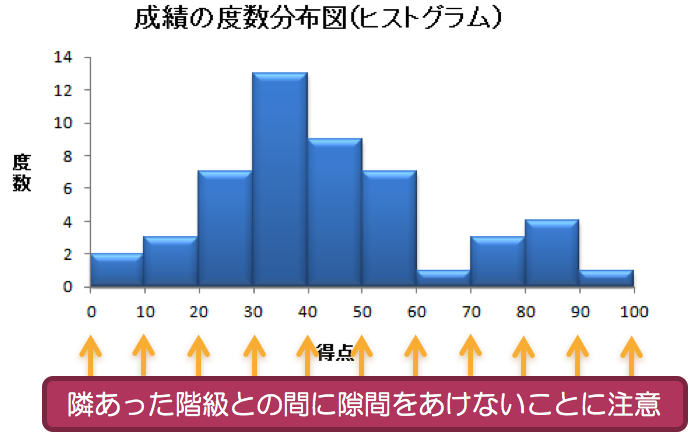
\includegraphics[width=0.5\textwidth,height=\textheight]{images/lec02/pic_hist_scores.png}
\caption{image of histogram}
\end{figure}

\begin{quote}
定義:スタージス(Sturges)の公式による階級の幅の決め方

\begin{enumerate}
\def\labelenumi{\arabic{enumi}.}
\tightlist
\item
  階級の数\(m\)を決定する:データ数が\(n\)のとき,適切な階級数\(m\)は
  \[
  m \approx 1+\frac{\log_{10} n}{\log_{10} 2} \approx 1+3.32 \log_{10} n
  \]
  なお,\(\approx\)は\textbf{ほぼ等しい}の意味。(参考:\(\log_{10} 2 \approx 0.301\))
\item
  階級の幅\(c\)を決定する:適切な級間隔\(c\)は
  \[
  c \approx \frac{x_{\max}-x_{\min}}{1+3.32 \log_{10} n}=\frac{\text{データの範囲}}{\text{階級数}}
  \]
\end{enumerate}
\end{quote}

\begin{itemize}
\tightlist
\item
  データの値の中で最も大きな値を\texttt{最大値(maximum)\textquotesingle{}\textquotesingle{},逆に最も小さな値を}最小値(minimum)'\,'とよびます
\item
  最大値と最小値の間隔を``データの範囲(range)'\,'とよびます
\end{itemize}

\begin{quote}
問題:学生の成績データ(スタージスの公式)
学生50人の成績データ(単位:点数)では最低点は5点,最高点は99点でした。スタージスの公式を使って,適切な階級数\(m\)と階級の幅\(c\)を求めて下さい
\end{quote}

\textbf{解答}

\begin{enumerate}
\def\labelenumi{\arabic{enumi}.}
\tightlist
\item
  スタージスの公式に必要な情報は次の通り
\end{enumerate}

\begin{longtable}[]{@{}lll@{}}
\toprule()
名称 & 記号 & 数値 \\
\midrule()
\endhead
データ数 & \(n\) & 50 \\
最大値 & \(x_{max}\) & 99 \\
最小値 & \(x_{min}\) & 5 \\
\bottomrule()
\end{longtable}

\begin{enumerate}
\def\labelenumi{\arabic{enumi}.}
\setcounter{enumi}{1}
\item
  適切な階級の数\(m\)は
  \[
  m 
  \approx 1+3.32 \times \log_{10} \mathop{50}_{\substack{\uparrow \\ n}}
  \approx 1+3.32 \times 1.699
  \approx 1+5.64 = 6.64
  \]
\item
  適切な級間隔\(c\)は
  \[
  c 
  \approx \frac{\text{データの範囲}}{\text{階級数}}
  \approx \frac{99-5}{7} 
  \approx 13
  \]
\end{enumerate}

\begin{quote}
階級の数の決め方の注意点
\end{quote}

\begin{enumerate}
\def\labelenumi{\arabic{enumi}.}
\tightlist
\item
  階級の「数」と「幅」は反比例の関係にある
\end{enumerate}

\begin{longtable}[]{@{}llll@{}}
\toprule()
階級の数 & 階級の幅 & ヒストグラム & 問題点 \\
\midrule()
\endhead
少なくする & 広くなる & 大雑把になる & 情報の喪失が大 \\
多くする & 狭くなる & 細かくなる & 情報を集約できない \\
\bottomrule()
\end{longtable}

\begin{enumerate}
\def\labelenumi{\arabic{enumi}.}
\setcounter{enumi}{1}
\item
  適切な階級の数と幅を決定するときにスタージスの公式を参考にするといい
\item
  次のような幅を設定することがポイント

  \begin{enumerate}
  \def\labelenumii{\arabic{enumii}.}
  \tightlist
  \item
    データ全体の傾向は損なわず、整理しやすい手頃な幅
  \item
    級間隔が直感的に分かりやすい幅
  \end{enumerate}
\end{enumerate}

\hypertarget{ux5ea6ux6570ux5206ux5e03ux8868ux304bux3089ux308fux304bux308bux3053ux3068}{%
\subsection{度数分布表からわかること}\label{ux5ea6ux6570ux5206ux5e03ux8868ux304bux3089ux308fux304bux308bux3053ux3068}}

\begin{quote}
問題:学生の成績データ(度数分布表の解釈)
先ほど作成した学生の成績データの\textbf{度数分布表}を参照しながら以下の値を求めて下さい

\begin{enumerate}
\def\labelenumi{\arabic{enumi}.}
\tightlist
\item
  点数が30点台の学生は何人いますか?
\item
  点数が30点台の学生は全体の何パーセントですか?
\item
  50点未満の学生は何人いますか?
\item
  50点未満の学生は何パーセントですか?
\end{enumerate}
\end{quote}

\textbf{解答}
1. 13人
2. 26パーセント
3. 34人
4. 68パーセント

\begin{quote}
問題:学生の成績データ(相対度数)
点数が31点から40点の学生は全体の何パーセントですか?
\end{quote}

\[
\text{30点台の階級の相対度数}
=\frac{\text{30点台の階級の度数}}{\text{全度数}}
=\frac{13}{50}=0.26
\]

\begin{quote}
定義:相対度数分布
\textbf{相対度数}の分布を表示したもの
\end{quote}

\begin{longtable}[]{@{}rrcl@{}}
\toprule()
階級(点) & 度数(人) & 相対度数 & \\
\midrule()
\endhead
0-9 & 2 & 0.04 & \(\leftarrow 2/50\) \\
10-19 & 3 & 0.06 & \(\leftarrow 3/50\) \\
20-29 & 7 & 0.14 & \\
30-39 & 13 & 0.26 & \(\leftarrow 13/50\) \\
40-49 & 9 & 0.18 & \\
50-59 & 7 & 0.14 & \\
60-69 & 1 & 0.02 & \\
70-79 & 3 & 0.06 & \\
80-89 & 4 & 0.08 & \\
90-99 & 1 & 0.02 & \\
合計 & 50 & 1.00 & \\
\bottomrule()
\end{longtable}

\hypertarget{ux30edux30fcux30ecux30f3ux30c4ux66f2ux7dda}{%
\chapter{ローレンツ曲線}\label{ux30edux30fcux30ecux30f3ux30c4ux66f2ux7dda}}

\begin{quote}
定義:(所得の)5分位階級
全ての世帯を所得の低い方から順番に並べ,それを世帯数で五等分して五つのグループを作った場合の各グループのことで,収入の低い方から順次第1,第2,第3,第4,第5分位階級とよぶ(参考:総務省,家計調査\textasciitilde 用語の解説 \url{http://www.stat.go.jp/data/kakei/kaisetsu.htm})
\end{quote}

\begin{quote}
問題:アメリカの1966年時点の所得の分布
次はアメリカの1966年時点の5分位階級別の所得の割合(\%)を示したデータです。コメントして下さい。
\end{quote}

\begin{longtable}[]{@{}llllll@{}}
\toprule()
所得階級 & 第1分位 & 第2分位 & 第3分位 & 第4分位 & 第5分位 \\
\midrule()
\endhead
1966年 & 5.6 & 12.4 & 17.7 & 23.8 & 40.5 \\
\bottomrule()
\end{longtable}

出所:US Department of Commerce, Statistical Abstract of the United States

\begin{quote}
定義:円グラフ(パイチャート)
360度の円を,100分比に応じて中心点から扇状に区切ったグラフ表現のこと。構成比を表すのに適したグラフ
\end{quote}

\begin{figure}
\centering
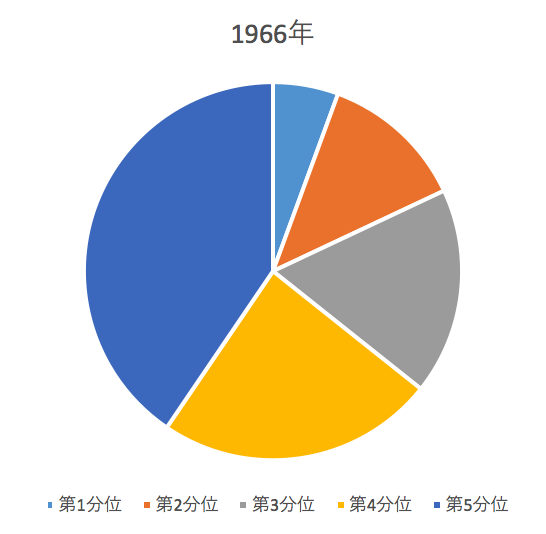
\includegraphics[width=0.5\textwidth,height=\textheight]{images/lec03/fig_us_income_dist1966.png}
\caption{image of histogram}
\end{figure}

\begin{quote}
問題:アメリカの1966年時点の所得の分布
世帯数と所得の累積比率を計算し,コメントして下さい
\end{quote}

\textbf{解答}

~~~~~~~~~\textbar{} 所得分配 \textbar{} 累積比率 \textbar{} 累積比率 \textbar{}\\
所得階級 \textbar{} 1966年 \textbar{} 世帯数 \textbar{} 所得 \textbar{}\\
--- \textbar{} --- \textbar{} --- \textbar{} --- \textbar{}\\
第1分位 \textbar{} 0.056 \textbar{} 0.200 \textbar{} 0.056 \textbar{}\\
第2分位 \textbar{} 0.124 \textbar{} 0.400 \textbar{} 0.180 \textbar{}\\
第3分位 \textbar{} 0.177 \textbar{} 0.600 \textbar{} 0.357 \textbar{}\\
第4分位 \textbar{} 0.238 \textbar{} 0.800 \textbar{} 0.595 \textbar{}\\
第5分位 \textbar{} 0.405 \textbar{} 1.000 \textbar{} 1.000 \textbar{}

\begin{itemize}
\tightlist
\item
  第1分位は所得全体の5.6\%
\item
  所得が低い方から6割の世帯(第3分位までの世帯)の所得は,全体の4割未満(35.7\%)
\item
  所得が多い上位20\%の世帯が,全所得の4割程度を獲得している
\end{itemize}

\begin{quote}
問題:アメリカの1966年時点の所得の分布
1966年時点のアメリカの所得分配は不平等のように思えます。では逆に,完全に平等な場合の,(1)円グラフ,(2)累積比率はどうなりますか
\end{quote}

\begin{figure}
\centering
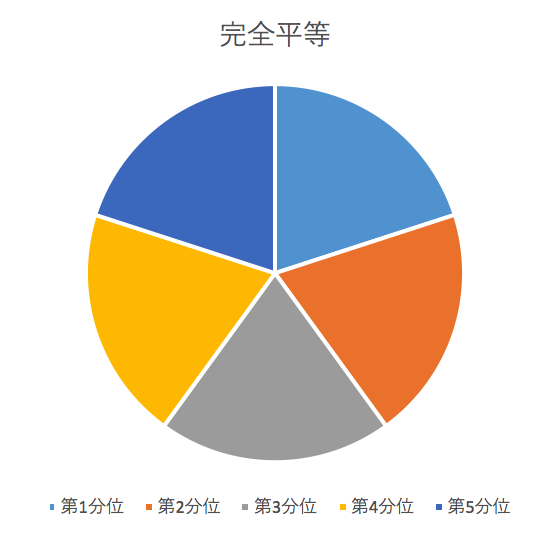
\includegraphics[width=0.5\textwidth,height=\textheight]{images/lec03/fig_income_dist_perfectly_equal.png}
\caption{image of histogram}
\end{figure}

\begin{quote}
問題:アメリカの1966年時点の所得の分布
所得分配の不平等度を的確に表す方法は?
\end{quote}

\begin{quote}
定義:ローレンツ曲線
ローレンツ曲線(Lorenz curve)は,所得分布や資産分布などの格差,不平等度,集中度を明らかにするための代表的な方法で,1905年にアメリカの統計学者ローレンツ(M.O.Lorenz)によって考案されました
\end{quote}

\begin{quote}
累積世帯比率と累積所得比率
\end{quote}

\hypertarget{ux30edux30fcux30ecux30f3ux30c4ux66f2ux7ddaux3068ux30b8ux30cbux4fc2ux6570}{%
\subsection{ローレンツ曲線とジニ係数}\label{ux30edux30fcux30ecux30f3ux30c4ux66f2ux7ddaux3068ux30b8ux30cbux4fc2ux6570}}

\begin{figure}
\centering
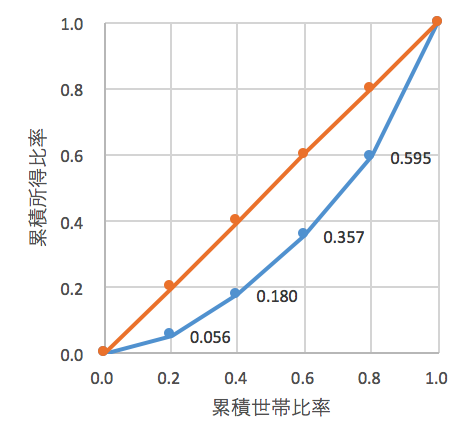
\includegraphics[width=0.5\textwidth,height=\textheight]{images/lec03/fig_us_lorenz1966.png}
\caption{image of histogram}
\end{figure}

\begin{quote}
ポイント

\begin{enumerate}
\def\labelenumi{\arabic{enumi}.}
\tightlist
\item
  青線が1966年のデータから計算した\textbf{ローレンツ曲線}です
\item
  オレンジ線を\textbf{完全平等線}とよびます
\item
  \textbf{所得分配が平等化}してくるとローレンツ曲線は完全平等線に\textbf{接近}します
\item
  オレンジと青の線の間の\textbf{領域が広いほど不平等度が高く}なります
\item
  2本の線に挟まれた\textbf{領域の面積の2倍の値をジニ係数}とよびます
\end{enumerate}
\end{quote}

\begin{quote}
確認問題:2005年のアメリカの所得分布
2005年の数値を使ってローレンツ曲線を描き,結果についてコメントして下さい
\end{quote}

\textbf{解答}

\begin{figure}
\centering
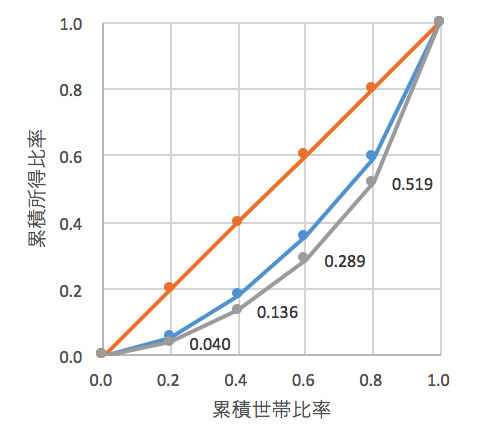
\includegraphics[width=0.5\textwidth,height=\textheight]{images/lec03/fig_us_lorenz2005.png}
\caption{image of histogram}
\end{figure}

\begin{itemize}
\tightlist
\item
  1969年から2005年にかけて,ローレンツ曲線は完全平等線からさらに離れている
\item
  このことから,1966年から2005年にかけて所得分布の不平等化が進んでいることがうかがわれる
\end{itemize}

\hypertarget{ux30b8ux30cbux4fc2ux6570}{%
\section{ジニ係数}\label{ux30b8ux30cbux4fc2ux6570}}

\begin{quote}
定義:ジニ係数

\begin{enumerate}
\def\labelenumi{\arabic{enumi}.}
\tightlist
\item
  ジニ係数(Gini coefficient)はローレンツ曲線のかたちを計測可能な指数にしたもので,(所得分配などの)分布の不平等度,集中度を示す指標です。
\item
  ジニ係数は\textbf{0から1のあいだの値}をとり,0に近いほど平等に近く,1に近いほど不平等度が大きいことを意味します
\end{enumerate}
\end{quote}

\begin{quote}
ジニ係数の計算方法

\begin{enumerate}
\def\labelenumi{\arabic{enumi}.}
\tightlist
\item
  完全平等線より右下の領域(領域A)の面積は0.5
\item
  ローレンツ曲線よりも右下の領域Bの面積を求める
\end{enumerate}
\end{quote}

\begin{align*}
\text{ジニ係数}
=(\text{領域Aの面積}-\text{領域Bの面積})\times 2
=1-\text{領域Bの面積}\times 2 
\end{align*}

\begin{quote}
\begin{enumerate}
\def\labelenumi{\arabic{enumi}.}
\setcounter{enumi}{2}
\tightlist
\item
  ローレンツ曲線よりも右下の領域の面積の計算方法
\end{enumerate}
\end{quote}

\begin{figure}
\centering
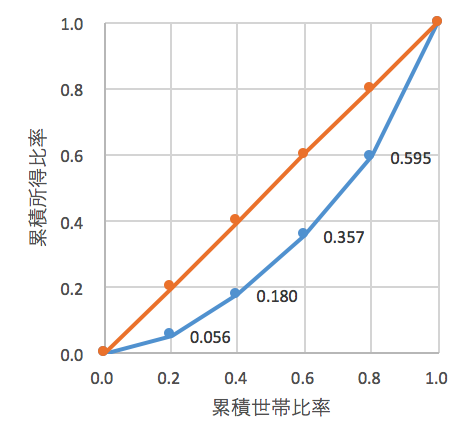
\includegraphics[width=0.5\textwidth,height=\textheight]{images/lec03/fig_us_lorenz1966.png}
\caption{image of histogram}
\end{figure}

\begin{itemize}
\tightlist
\item
  領域を5分割し,三角形と台形の面積を求め,合計します
\end{itemize}

\begin{align*} 
&\tfrac{1}{2} \times \mathop{0.056}_{\substack{\uparrow \\ \text{底辺}}} \times \mathop{0.2}_{\substack{\uparrow \\ \text{高さ}}} \\
&+\tfrac{1}{2} \times (0.056+0.180) \times 0.2 \\
&+\tfrac{1}{2} \times (0.180+0.357) \times 0.2 \\
&+\tfrac{1}{2} \times (0.357+0.595) \times 0.2 \\
&+\tfrac{1}{2} \times (
\mathop{0.595}_{\substack{\uparrow \\ \text{上底}}}
+
\mathop{1.000}_{\substack{\uparrow \\ \text{下底}}}
) \times 
\mathop{0.2}_{\substack{\uparrow \\ \text{高さ}}} \\
&=0.3376
\end{align*}

\begin{enumerate}
\def\labelenumi{\arabic{enumi}.}
\setcounter{enumi}{3}
\item
  よって1969年のジニ係数は
  \begin{align*}
  \text{ジニ係数}=1-0.3376\times 2=0.3248
  \end{align*}
\item
  領域Bの計算のコツ
\end{enumerate}

\begin{itemize}
\item
  今回の例では,5分位の世帯比率を使っているため,累積世帯比率は20\%ずつ等間隔で増加します。そのため面積を計算するときの``高さ'\,'はすべて0.2です
\item
  さらに,三角形と台形の公式では\(\tfrac{1}{2}\)が共通です
\item
  これらの共通項を括り出せば
\end{itemize}

\begin{align*} 
&\tfrac{1}{2} \times \mathop{0.2}_{\substack{\uparrow \\ \text{高さ}}} \times 
\{ 0.056+ (0.056+0.180)+ (0.180+0.357) \\
&\qquad\qquad+(0.357+0.595)+(0.595+1.000) \} \\
&=0.3376
\end{align*}

\begin{quote}
確認問題:2005年のアメリカの所得分布
2005年の数値を使ってジニ係数を計算して下さい
\end{quote}

\textbf{解答}

\begin{enumerate}
\def\labelenumi{\arabic{enumi}.}
\item
  領域Bの面積は
  \begin{align*}
  \text{領域Bの面積}
  &=\tfrac{1}{2} \times \mathop{0.2}_{\substack{\uparrow \\ \text{高さ}}} \times 
  \{ 0.040+ (0.040+0.136) \\
  &\qquad\qquad+(0.136+0.289)+(0.289+0.519) \\
  &\qquad\qquad+(0.519+1.000) \} \\
  &=0.2968
  \end{align*}
\item
  したがって2005年のジニ係数は
  \begin{align*}
  \text{ジニ係数}
  =1-2 \times 0.2968
  =0.4064
  \end{align*}
\item
  解釈:ジニ係数の値は0.3248(1969年)から0.4064(2005年)へ上昇しており,所得分配の不平等化がすすんだ
\end{enumerate}

\hypertarget{ux30b8ux30cbux4fc2ux6570ux306eux5225ux306eux5fdcux7528ux4f8b}{%
\chapter{ジニ係数の別の応用例}\label{ux30b8ux30cbux4fc2ux6570ux306eux5225ux306eux5fdcux7528ux4f8b}}

\begin{figure}
\centering
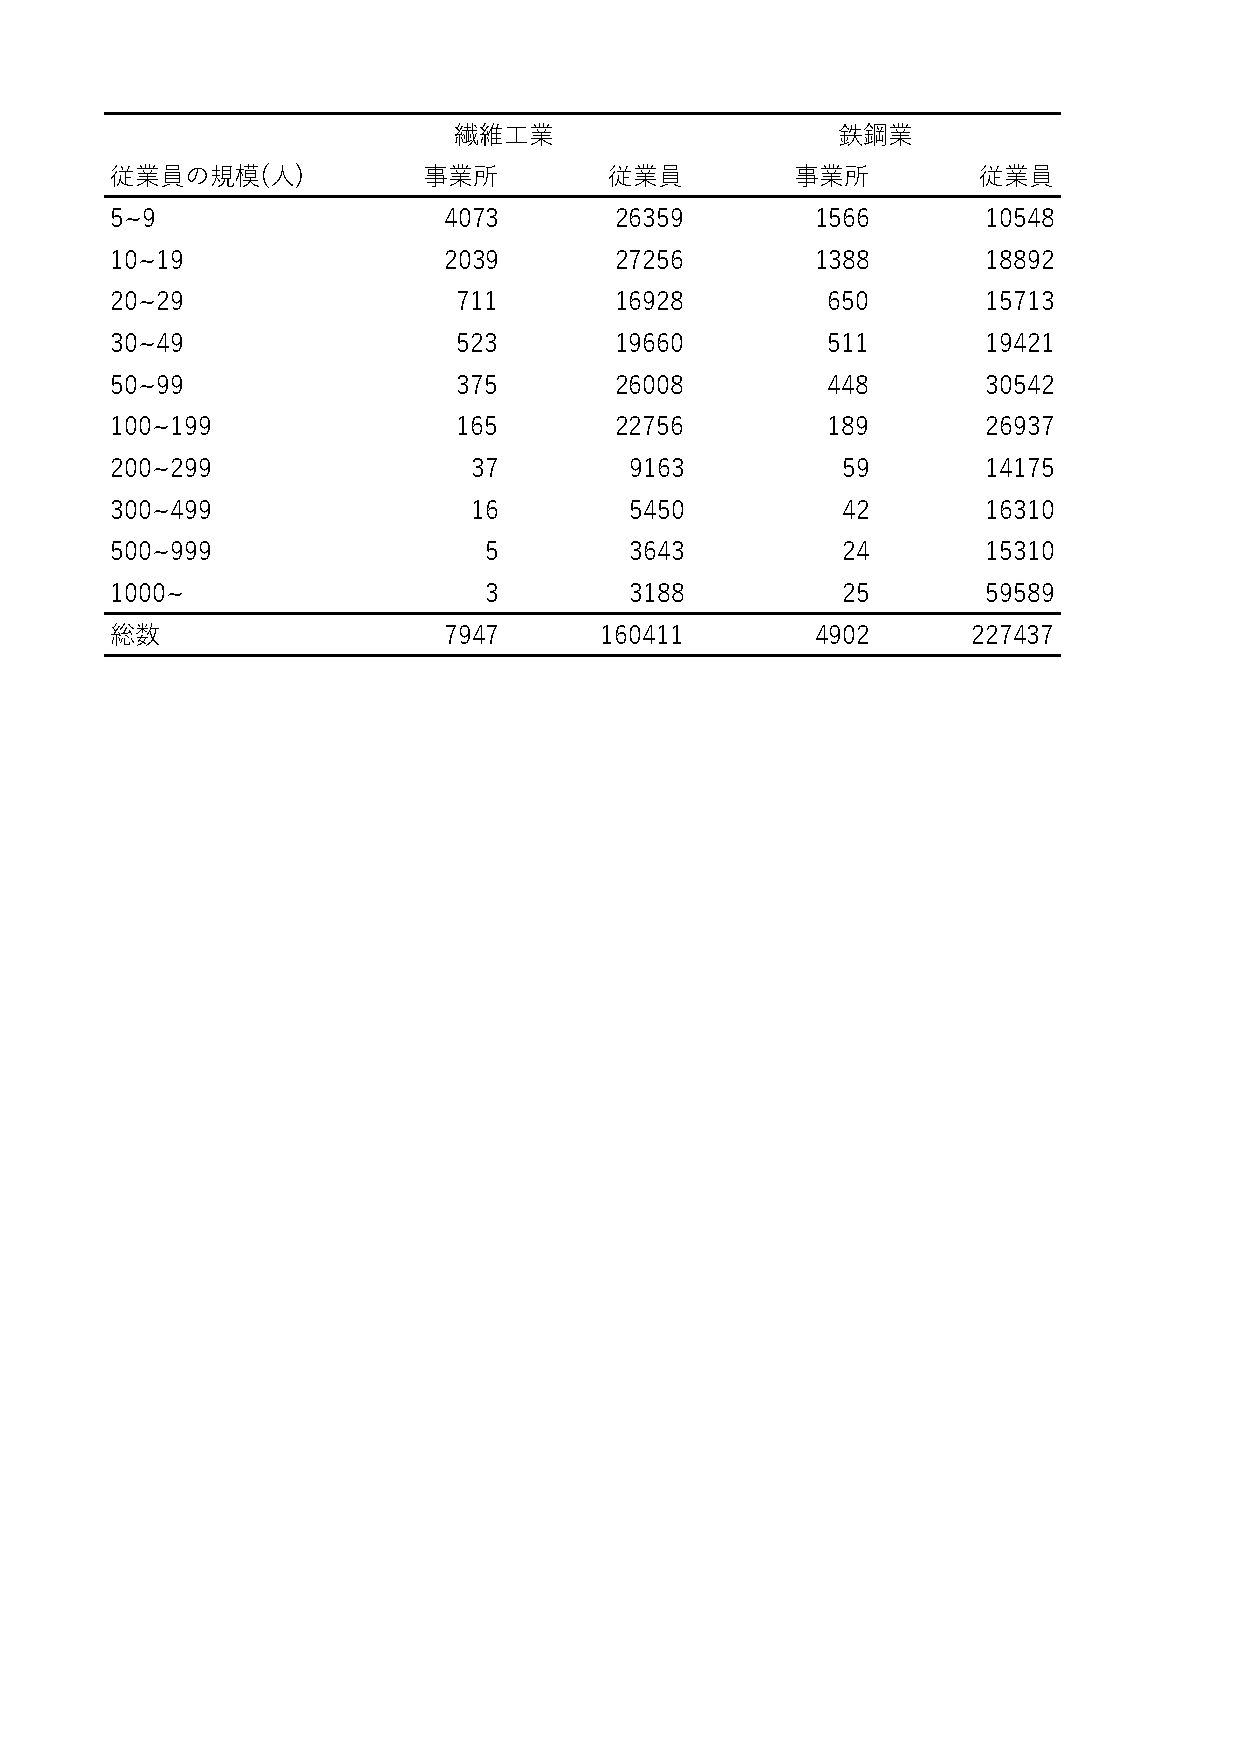
\includegraphics[width=1\textwidth,height=\textheight]{images/lec04/tab_textile_steel1.pdf}
\caption{image of histogram}
\end{figure}

\begin{itemize}
\tightlist
\item
  事業所数と従業員数の累積相対比率を計算すると次表のようになります
\end{itemize}

\begin{figure}
\centering
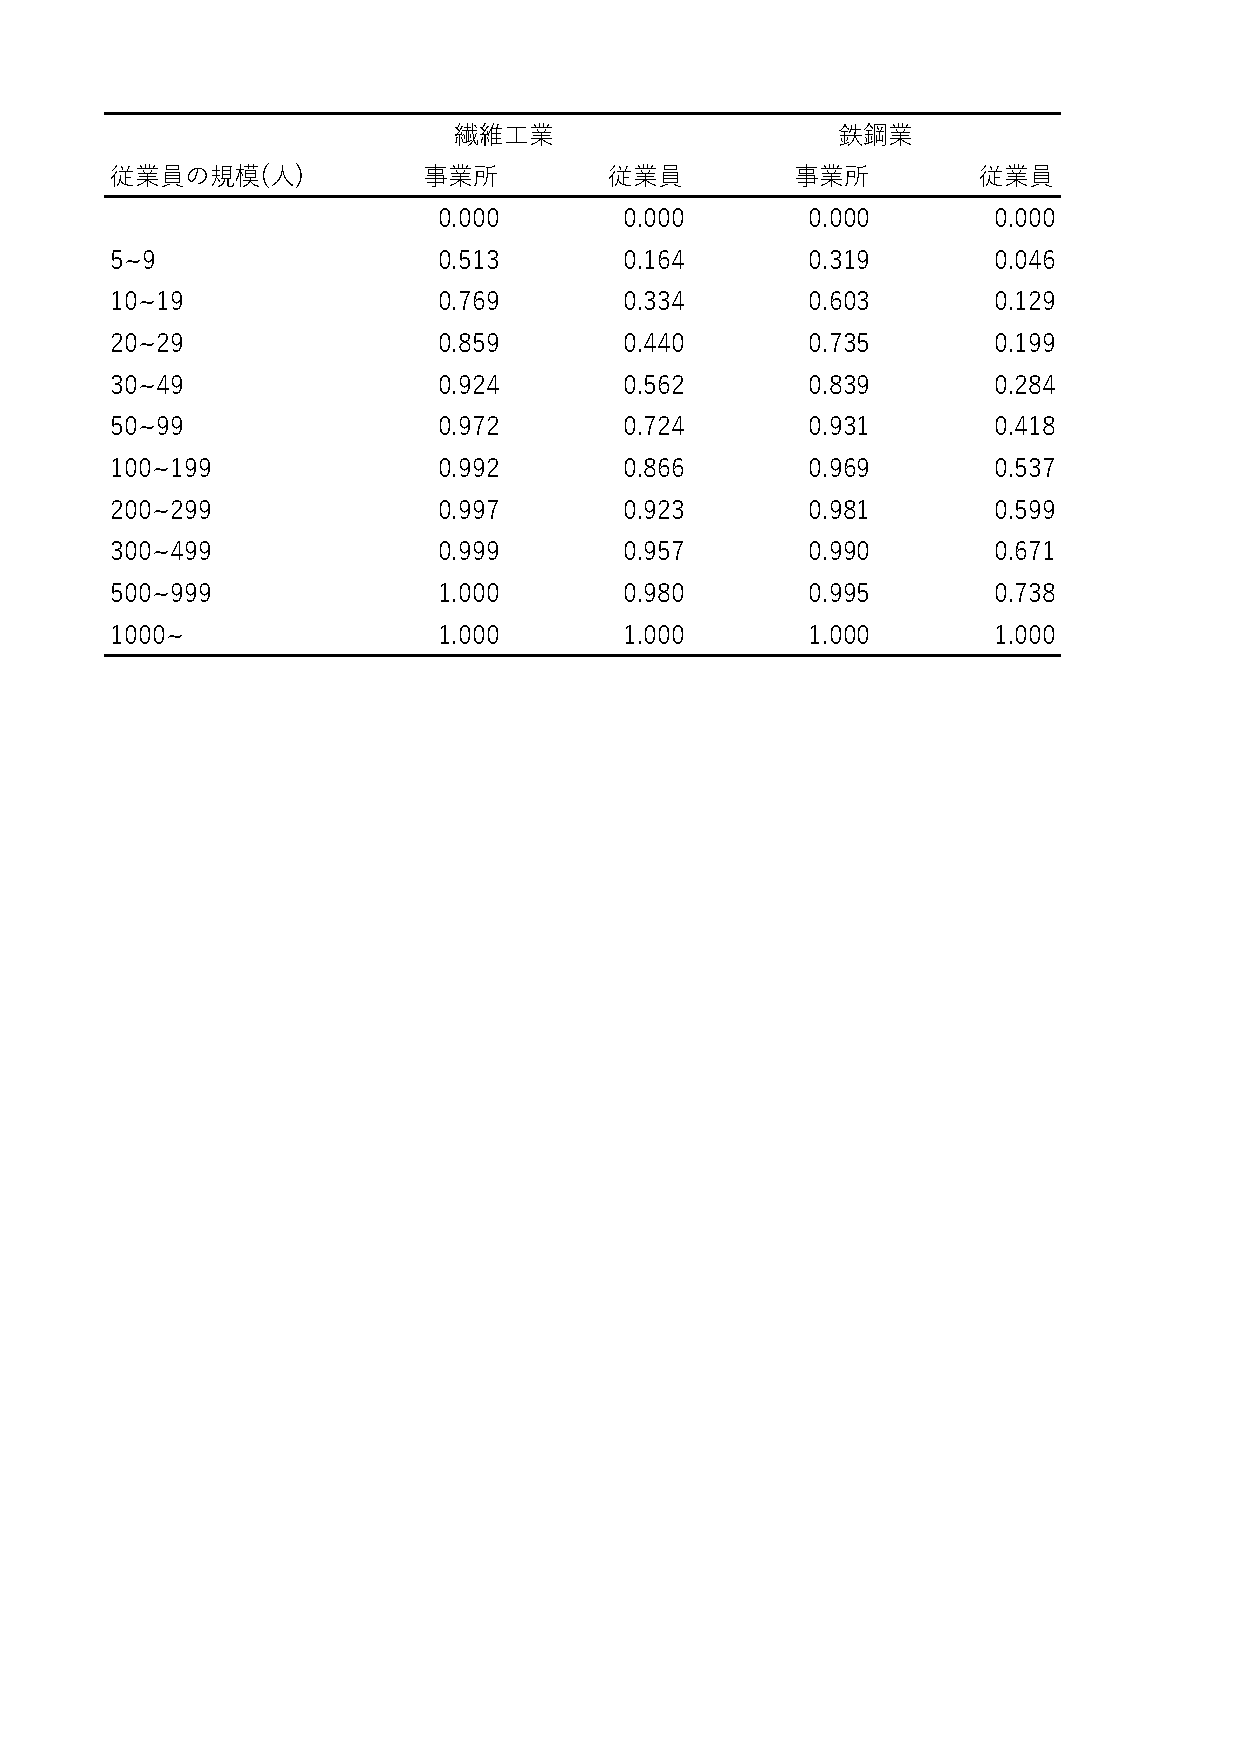
\includegraphics[width=1\textwidth,height=\textheight]{images/lec04/tab_textile_steel2.pdf}
\caption{image of histogram}
\end{figure}

\begin{itemize}
\tightlist
\item
  ローレンツ曲線は次のようになります
\end{itemize}

\begin{figure}
\centering
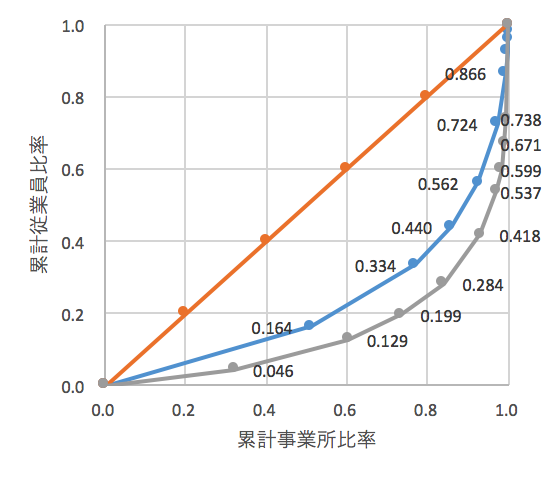
\includegraphics[width=1\textwidth,height=\textheight]{images/lec04/fig_textile_steel.png}
\caption{image of histogram}
\end{figure}

\begin{quote}
問題

\begin{itemize}
\tightlist
\item
  繊維工業はどちらでしょうか?
\item
  どちらの方が集中度が高いでしょうか?また直感とあっていますか?
\end{itemize}

(解答:ジニ係数は繊維が0.5448,鉄鋼業が0.7003)
\end{quote}

\begin{itemize}
\tightlist
\item
  ヨコ軸の増加幅が等間隔でないため``高さ'\,'の値がバラバラです
\item
  しかし必要な領域の面積は(若干面倒ですが)以前の例と同じ考え方で計算できます
\end{itemize}

\hypertarget{ux30b7ux30b0ux30deux8a18ux53f7}{%
\section{シグマ記号}\label{ux30b7ux30b0ux30deux8a18ux53f7}}

\begin{quote}
重要な3つのルール

\begin{itemize}
\item
  ルール1
  \begin{align*}
  \sum_{i=1}^n (X_i+c)=\sum_{i=1}^n X_i+nc
  \end{align*}
\item
  ルール2
  \begin{align*}
  \sum_{i=1}^n c X_i=c \sum_{i=1}^n X_i
  \end{align*}
\item
  ルール3
  \begin{align*}
  \sum_{i=1}^n (a X_i+b)=a \sum_{i=1}^n X_i +nb
  \end{align*}
\end{itemize}
\end{quote}

\textbf{ルール1の確認}

一般的には大きさが\(n\)の標本 \(\{ X_i \}=\{ X_1,X_2,\cdots,X_n \}\)のそれぞれのデータに定数\(c\)を加えた新しいデータ \(\{ X_i+c \}\)の和は
\begin{align}
\sum_{i=1}^n (X_i+c)
&=(X_1+c)+(X_2+c)+\cdots+(X_n+c) \nonumber \\
&=(X_1+X_2+\cdots+X_n)+\underbrace{(c+c+\cdots+c)}_{\text{$n$個の$c$の合計}} \nonumber \\
&=\sum_{i=1}^n X_i+nc \label{(2.15)}
\end{align}
になります。

\textbf{ルール2の確認}

一般的には大きさが\(n\)の標本 \(\{ X_i \}=\{ X_1,X_2,\cdots,X_n \}\)のそれぞれのデータを\(c\)倍した新しいデータ \(\{ c X_i \}\)の和は
\begin{align}
\sum_{i=1}^n c X_i
&=c X_1+c X_2+\cdots+c X_n \nonumber \\
&=c (X_1+X_2+\cdots+X_n) \nonumber \\
&=c \sum_{i=1}^n X_i \label{(2.17)}
\end{align}
になります。

\textbf{ルール3の確認}

式(\ref{(2.15)})と式(\ref{(2.17)})を組合せると,大きさ\(n\)の標本 \(\{ X_i \}\)のそれぞれのデータを\(a\)倍し,さらにそれぞれに\(b\)を足しあわせた新しいデータ\(\{ aX_i+b \}\)の和を次のように計算できます。
\begin{align}
\sum_{i=1}^n (a X_i+b)
&=(a X_1+b)+(a X_2+b)+\cdots+(a X_n+b) \nonumber \\
&=\underbrace{(aX_1+aX_2+\cdots+aX_n)}_{a (X_1+X_2+\cdots+X_n)}+\underbrace{(b+b+\cdots+b)}_{\text{$n$個の$b$の合計}} \nonumber \\
&=a \sum_{i=1}^n X_i+nb \label{(2.18)}
\end{align}

\begin{quote}
ジニ係数と5分位(Gini\_Quintile2021.tex)
\end{quote}

\begin{enumerate}
\def\labelenumi{\arabic{enumi}.}
\tightlist
\item
  世帯を所得の低い方から順に並べ,世帯数で5等分し,それぞれを第I,第II,第III,第IV,第V五分位階級とよぶ。ここで横軸に累積世帯比率,縦軸に累積所得比率をとった座標平面において,次のローレンツ曲線のジニ係数を記号で表現する。
\end{enumerate}

\begin{figure}
\centering
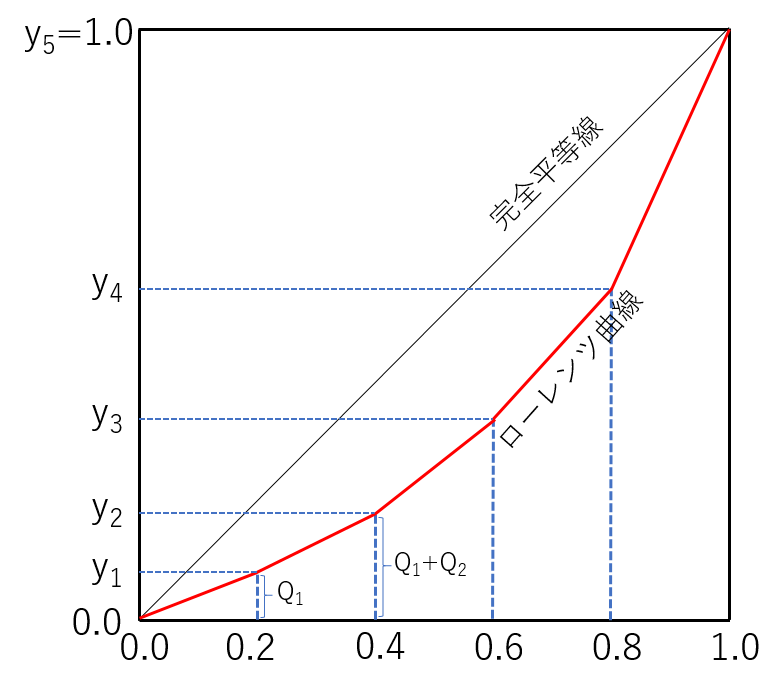
\includegraphics[width=0.8\textwidth,height=\textheight]{images/lec04/GINI_GRAPH.png}
\caption{image of histogram}
\end{figure}

\begin{longtable}[]{@{}cccc@{}}
\toprule()
所得階級 & 所得分配 & 世帯数 & 所得 \\
\midrule()
\endhead
第I 五分位階級 & \(Q_1\) & 0.2 & \(y_1\) \\
第II 五分位階級 & \(Q_2\) & 0.4 & \(y_2\) \\
第III 五分位階級 & \(Q_3\) & 0.6 & \(y_3\) \\
第IV 五分位階級 & \(Q_4\) & 0.8 & \(y_4\) \\
第V 五分位階級 & \(Q_5\) & 1.0 & \(y_5\) \\
\bottomrule()
\end{longtable}

\begin{enumerate}
\def\labelenumi{\arabic{enumi}.}
\setcounter{enumi}{2}
\tightlist
\item
  \(Q_i\)は第\(i\)階級の所得割合。\(y_i\)は第\(i\)階級までの累積値。
\end{enumerate}

\begin{itemize}
\tightlist
\item
  ローレンツ曲線よりも右下の領域の面積はそれぞれ
\end{itemize}

\begin{align*}
\text{第I階級の部分の面積}
&=
\text{底辺}\times\text{高さ}\div 2 \\
&=
\mathop{y_1}_{\text{底辺}} \times \mathop{0.2}_{\text{高さ}} \times \frac{1}{2} =0.1 \times y_1
\end{align*}

\begin{align*}
\text{第II階級の部分の面積}
&=
(\text{上底}+\text{下底})\times\text{高さ}\div 2
=(y_1+y_2) \times 0.2 \times \frac{1}{2}=0.1 \times (y_1+y_2)
\end{align*}

\begin{align*}
\text{第III階級の部分の面積}
&
=
(y_2+y_3) \times 0.2 \times \frac{1}{2}=0.1 \times (y_2+y_3)
\end{align*}

\begin{align*}
\text{第IV階級の部分の面積}
&
=
(y_3+y_4) \times 0.2 \times \frac{1}{2}=0.1 \times (y_3+y_4)
\end{align*}

\begin{align*}
\text{第V階級の部分の面積}
&
=(y_4+y_5) \times 0.2 \times \frac{1}{2} =0.1 \times (y_4+1)
\end{align*}

\begin{itemize}
\tightlist
\item
  以上を合計すれば,ローレンツ曲線よりも右下の領域(領域B)の面積は
\end{itemize}

\begin{align*}
\text{領域Bの面積}&=
0.1 \times y_1
+0.1 \times (y_1+y_2)
+0.1 \times (y_2+y_3)
+0.1 \times (y_3+y_4)
+0.1 \times (y_4+1) \\
&=0.1 \times \{ y_1+(y_1+y_2)+(y_2+y_3)+(y_3+y_4)+(y_4+1) \} \\
&=0.1 \times ( 2y_1+2 y_2+2 y_3+2 y_4 +1 )
\end{align*}

\begin{itemize}
\tightlist
\item
  ジニ係数は,完全平等線より右下の領域の面積(\(1/2\))からローレンツ曲線よりも右下の領域の面積を引き,2倍したものなので
\end{itemize}

\begin{align}
\text{Gini係数}
&=\underbrace{2 \times 0.5}_{\text{領域Aの2倍}}
-
\underbrace{2 \times 0.1 \times ( 2y_1+2 y_2+2 y_3+2 y_4 +1 )}_{\text{領域Bの2倍}} \nonumber \\
&=1-(0.4y_1+0.4y_2+0.4y_3+0.4y_4+0.2)  \nonumber \\
&=0.8-0.4 \times ( y_1+y_2+y_3+y_4)  \label{gini_eq1}
\end{align}

\begin{itemize}
\tightlist
\item
  ここで\(y\)と\(Q\)のあいだには次の関係があるので
\end{itemize}

\begin{align*}
y_1&=Q_1 \\
y_2&=Q_1+Q_2 \\
y_3&=Q_1+Q_2+Q_3 \\
y_4&=Q_1+Q_2+Q_3+Q_4
\end{align*}
このことから
\begin{align}
y_1+y_2+y_3+y_4=4 Q_1+3 Q_2+2 Q_3+Q_4 \label{gini_eq2}
\end{align}

\begin{itemize}
\tightlist
\item
  したがって(\ref{gini_eq1})式と(\ref{gini_eq2})式から、ジニ係数は次の式により三角形や台形の面積を計算することなく,各五分位の所得分配の値からも直接計算できる。
\end{itemize}

\begin{align}
\text{Gini係数}
&=0.8-0.4 \times ( 4 Q_1+3 Q_2+2 Q_3+Q_4 ) \label{gini_eq3}
\end{align}

\begin{quote}
問題:次は1966年時点のアメリカの所得分布です。(\ref{gini_eq3})式を使ってジニ係数の値を求めて下さい。
\end{quote}

\begin{quote}
解答:ジニ係数は

\begin{align*}
\text{Gini係数}
&=0.8-0.4 \times ( 4 Q_1+3 Q_2+2 Q_3+Q_4 ) \\
&=0.8-0.4 \times ( 4 \times 0.056+3 \times 0.124+2 \times 0.177+0.238 ) \\
&=0.8-0.4 \times ( 0.224+0.372+0.354+0.238 ) \\
&=0.8-0.4 \times 1.188 =0.8-0.4752=0.3248
\end{align*}
\end{quote}

\begin{quote}
参考文献:
Barro, R.J. (1999), Inequality, Growth and Investment, NBER Working Paper 7038.
\end{quote}

\begin{quote}
応用例:偏差\(\{ X_i-\bar{X} \}\)の合計
\end{quote}

大きさ\(n\)の標本から計算した標本平均を
\begin{align*}
\bar{X}=\frac{1}{n} \sum_{i=1}^n X_i
\end{align*}
で表します。ここで標本平均はただ1つの値しかとらないので定数です。例えば\(c=-\bar{X}\)として式(\ref{(2.15)})のルールを適用すれば,偏差\(\{ X_i-\bar{X} \}\)の合計は以下のようになります。
\begin{align*}
\sum_{i=1}^n (X_i-\bar{X})
&=(X_1-\bar{X})+(X_2-\bar{X})+\cdots+(X_n-\bar{X}) \\
&=\underbrace{(X_1+X_2+\cdots+X_n)}_{\sum_{i=1}^n X_i}
+\underbrace{\{ (-\bar{X})+(-\bar{X})+\cdots+(-\bar{X}) \}}_{\text{$n$個の$-\bar{X}$の合計}}
\end{align*}
ここで
\begin{align*}
\bar{X}=\frac{1}{n}\sum_{i=1}^n X_i
\qquad \text{を書き換えれば} \qquad
\sum_{i=1}^n X_i=n \bar{X}
\end{align*}
となることに注目して下さい。したがって
\begin{align*}
\sum_{i=1}^n (X_i-\bar{X})
&=\underbrace{(X_1+X_2+\cdots+X_n)}_{\sum_{i=1}^n X_i}
+\underbrace{\{ (-\bar{X})+(-\bar{X})+\cdots+(-\bar{X}) \}}_{\text{$n$個の$-\bar{X}$の合計}} \\
&=\sum_{i=1}^n X_i-n \bar{X} \\
&=0
\end{align*}
となります。つまり「偏差の合計はゼロ」になります。

\hypertarget{ux5206ux5e03ux306eux4ee3ux8868ux5024}{%
\chapter{分布の代表値}\label{ux5206ux5e03ux306eux4ee3ux8868ux5024}}

\hypertarget{ux7b97ux8853ux5e73ux5747}{%
\section{算術平均}\label{ux7b97ux8853ux5e73ux5747}}

\begin{quote}
問題1:平均年収の計算
5人の年収が、それぞれ100万円、300万円、600万円、900万円、1200万円のとき、この5 人の平均年収はいくらですか?
\end{quote}

番号 \textbar{} 1 \textbar{} 2 \textbar{} 3 \textbar{} 4 \textbar{} 5 \textbar{}\\
記号 \textbar{} \(x_1\) \textbar{} \(x_2\) \textbar{} \(x_3\) \textbar{} \(x_4\) \textbar{} \(x_5\) \textbar{}

\textbar--\textbar--\textbar--\textbar--\textbar--\textbar--\textbar{}
\textbar{} 年収(万円) \textbar{} 100 \textbar{} 300 \textbar{} 600 \textbar{} 900 \textbar{} 1200 \textbar{}

\begin{quote}
解答

平均年収は
\begin{align*}
\text{平均年収}=\frac{100+300+600+900+1200}{5}=620(\text{万円})
\end{align*}
\end{quote}

\begin{quote}
定義:算術平均

\begin{itemize}
\tightlist
\item
  \(n\)個の観測値を\(x_1,x_2,\dots,x_n\)と表すとき、それらの算術平均は
\end{itemize}

\begin{eqnarray*}
\bar{x}=\frac{x_1+x_2+\cdots+x_n}{n}=\frac{1}{n}\sum_{i=1}^n x_i
\end{eqnarray*}
\end{quote}

\begin{itemize}
\tightlist
\item
  先ほどの例では,年収を変数\(x\)で表し,番号を添字にするならば(例:1番目の人の年収を\(x_1\)という具合に表現する)
  \begin{align*}
  \bar{x}=\frac{x_1+x_2+x_3+x_4+x_5}{5}=\frac{1}{5}\sum_{i=1}^5 x_i
  \end{align*}
\end{itemize}

\begin{quote}
特徴:算術平均の重要な性質

\begin{enumerate}
\def\labelenumi{\arabic{enumi}.}
\tightlist
\item
  長所

  \begin{enumerate}
  \item すべての分布に常に存在する
  \item 唯一無二の平均値がえられる
  \item 計算が簡単
  \item すべてのデータを用いる
  \item 意味(=``データの重心'')が明瞭
  \end{enumerate}
\item
  短所

  \begin{enumerate}
  \item 例外値(外れ値)の影響を非常に受ける(次のスライドを参照)
  \item 適切な代表値でない場合がある
  \end{enumerate}
\item
  補足:算術平均の重要な性質
\end{enumerate}

\begin{itemize}
\tightlist
\item
  算術平均からの\textbf{偏差の和は常に0}になる
\item
  算術平均はデータの一次変換を保持する
\item
  \textbf{算術平均は偏差平方和を最小にするような値}である
\end{itemize}
\end{quote}

\begin{quote}
問題2:平均月給
以下の数値はある会社の全社員10名の月給で,10人の平均月給は30万円です。
\begin{align*}
\text{24~~12~~80~~16~~28~~16~~32~~16~~52~~24~(単位:万円)}
\end{align*}
平均月給はこのグループの給与分布の代表値と言えるでしょうか?
\end{quote}

\begin{quote}
解答
* 平均月収30万円は左右をバランスさせる点の値ですが,この場合では代表値とは言い難いでしょう
\end{quote}

\hypertarget{ux4e2dux592eux5024}{%
\section{中央値}\label{ux4e2dux592eux5024}}

\begin{quote}
定義:中央値
\end{quote}

\begin{itemize}
\item
  中央値とは観測値を大きさの順にならべたとき、その中央に位置するデータの値のこと。中位数,メディアン(median)。
\item
  中央値の求め方
\end{itemize}

\begin{enumerate}
\def\labelenumi{\arabic{enumi}.}
\tightlist
\item
  \(n\)が奇数ならば、\((n+1)/2\)番目のデータの値
\item
  \(n\)が偶数ならば、\(n/2\)番目と \(n/2+1\)番目のデータの値の平均値
\end{enumerate}

\begin{itemize}
\tightlist
\item
  算術平均と中央値の特徴の違い
\end{itemize}

\begin{enumerate}
\def\labelenumi{\arabic{enumi}.}
\tightlist
\item
  算術平均:すべてのデータの値を用いる
\item
  中央値:順序さえ決まったら、真ん中の値だけが問題となるので、他のデータの値は関係ない
\end{enumerate}

\begin{quote}
特徴:中央値の特徴
\end{quote}

\begin{enumerate}
\def\labelenumi{\arabic{enumi}.}
\tightlist
\item
  長所
\end{enumerate}

\begin{itemize}
\tightlist
\item
  外れ値(例外値、極端値、Outlier)の影響を受けない
\item
  常に唯一無二の中央値が存在する
\item
  煩雑な計算を必要としない
\end{itemize}

\begin{enumerate}
\def\labelenumi{\arabic{enumi}.}
\setcounter{enumi}{1}
\tightlist
\item
  短所
\end{enumerate}

\begin{itemize}
\tightlist
\item
  大量のデータに序列をつけるのは簡単ではない
\item
  すべてのデータを用いる訳ではない
\end{itemize}

\begin{quote}
問題3:算術平均と中央値
4つのクラス(A,B,C,D)で試験を行ったときの学生の成績が次のように得られました。

\begin{center}
A: 3,4,5,6,7(点)~~~~B: 1,3,5,7,9(点) \\
C: 0,4,5,6,10(点)~~~D: 0,1,5,9,10(点)
\end{center}

各クラスの平均\%(\(\bar{x}_A,\bar{x}_B,\bar{x}_C,\bar{x}_D\))
と中央値\%(\(Me_A,Me_B,Me_C,Me_D\))
を求めて下さい
\end{quote}

\begin{quote}
解答
\end{quote}

\begin{quote}
問題4:算術平均と中央値との大きな違い

算術平均と中央値との大きな違いは何でしょう?
\end{quote}

\begin{quote}
解答

\begin{itemize}
\tightlist
\item
  算術平均:すべてのデータの値を用いる
\item
  中央値:順序さえ決まったら、真ん中の値だけが問題となるので、他のデータの値は関係ない
\end{itemize}
\end{quote}

\hypertarget{ux6700ux983bux5024}{%
\section{最頻値}\label{ux6700ux983bux5024}}

\begin{quote}
定義:最頻値

最も多く観測されたデータの値のこと。モード(mode)。
\end{quote}

\begin{quote}
特徴:最頻値の特徴

\begin{enumerate}
\def\labelenumi{\arabic{enumi}.}
\tightlist
\item
  長所
\end{enumerate}

\begin{itemize}
\tightlist
\item
  外れ値(例外値、極端値、Outlier)の影響を受けない
\item
  煩雑な計算を必要としない
\end{itemize}

\begin{enumerate}
\def\labelenumi{\arabic{enumi}.}
\setcounter{enumi}{1}
\tightlist
\item
  短所
\end{enumerate}

\begin{itemize}
\tightlist
\item
  存在しないことがある
\item
  唯一無二でないことがある
\end{itemize}
\end{quote}

\begin{quote}
問題5:最頻値について

最頻値が存在しない場合とは,どんな場合でしょう?具体例をあげて下さい
\end{quote}

\begin{quote}
解答

\begin{itemize}
\tightlist
\item
  所得分布を分析するとき,実際の金額そのものをそのまま利用するならば,まったく同じ金額になる可能性は極めて低いので
\item
  階級幅を設けて度数分布表を作成した場合でも,異なる複数の階級の度数が同じになることがある
\end{itemize}
\end{quote}

\hypertarget{ux5e73ux5747ux5024ux4e2dux592eux5024ux6700ux983bux5024ux306eux95a2ux4fc2}{%
\section{平均値・中央値・最頻値の関係}\label{ux5e73ux5747ux5024ux4e2dux592eux5024ux6700ux983bux5024ux306eux95a2ux4fc2}}

参考文献 宮川公男(2016)『基本統計学{[}第3版{]}』有斐閣(序章)

\hypertarget{ux305dux306eux4ed6ux306eux7d71ux8a08ux91cf}{%
\chapter{その他の統計量}\label{ux305dux306eux4ed6ux306eux7d71ux8a08ux91cf}}

\begin{quote}
問題1:測定値の標準誤差の比較について

2つのグループ(XとY)が,異なるある2地点間の距離を100回ずつ測量して得たデータについて,標準誤差を計算したところ以下のようになった。

\begin{itemize}
\tightlist
\item
  Xグループ:地点Aと地点Bの測定の標準誤差は1m
\item
  Yグループ:地点Cと地点Dの測定の標準誤差は5mm
\end{itemize}

どちらのグループの測量の方が正確と言えるだろうか?
\end{quote}

\begin{quote}
問題2:測定値の標準誤差の比較について

Xグループが測定した区間(地点Aと地点B)の距離はおよそ1000m,これに対してYグループが測定した区間(地点Cと地点D)の距離は約1mだった。
どちらのグループの測量の方が正確と言えるだろうか?
\end{quote}

\begin{quote}
問題2:測定値の標準誤差の比較について

Xグループが測定した区間(地点Aと地点B)の距離はおよそ1000m,これに対してYグループが測定した区間(地点Cと地点D)の距離は約1mだった。
どちらのグループの測量の方が正確と言えるだろうか?
\end{quote}

\begin{quote}
解答

\begin{itemize}
\tightlist
\item
  前者は1000mに対して1mのばらつき,後者は1mに対して5mmのばらつきなので,「ばらつきの相対的大きさ」は
\end{itemize}

\begin{align*}
&\text{Xグループの場合}=\frac{1}{1000}=0.001 \\
&\text{Yグループの場合}=\frac{5}{1000}=0.005
\end{align*}
したがって前者の方が正確な測定と言える
\end{quote}

\begin{quote}
定義:変動係数(coefficient of variation)

標準偏差を算術平均で割ったもので
\begin{align*}
\text{変動係数(CV)}=\frac{\text{sd}(x)}{\bar{x}}=\frac{x\text{の標準偏差}}{x\text{の算術平均}}
\end{align*}
なお,使用するデータはすべて正。算術平均が0や0に近い場合,変動係数が計算できない,あるいは曖昧な尺度になるので注意が必要です
\end{quote}

\begin{quote}
問題3:為替レートの変動

次の表は1991年第1四半期から1996年第1四半期の期間の日本・ドイツ・フランスの為替レート(対ドル)の値です(抜粋)。
\end{quote}

変動リスクが一番高いと思われる通貨はどれですか? \% その理由も述べて下さい。

\begin{quote}
解答

\begin{itemize}
\tightlist
\item
  各国の通貨は単位が異なり,また水準も大きく異なるため,単純に標準偏差を比較しただけではどの通貨の変動が最も大きいのか,は判断できません
\item
  そこで,変動係数を計算します
\end{itemize}
\end{quote}

\begin{itemize}
\tightlist
\item
  このことから,日本,ドイツ,フランスの順に相対的分散度が大きいことがわかります
\end{itemize}

\begin{quote}
問題6:テストの成績\textasciitilde(平均と中央値)
\end{quote}

\begin{quote}
問題7:各統計量の特徴は?
\end{quote}

\begin{quote}
問題8:1年間に読んだ本の冊数\textasciitilde(範囲と四分位範囲)
\end{quote}

\begin{quote}
問題9:平均絶対偏差の計算

次の数値について平均絶対偏差を求めて下さい。
\end{quote}

\begin{quote}
解答

\begin{itemize}
\item
  まず平均を求めると
  \begin{align*}
  \bar{x}=\frac{1}{6}(3+2+6+1+5+7)=\frac{24}{6}=4
  \end{align*}
\item
  「平均からの偏差」の絶対値を平均するので
  \begin{align*}
  \text{MAD}
  &=\frac{1}{6}(|3-4|+|2-4|+|6-4|+|1-4|+|5-4|+|7-4|) \\
  &=\frac{1}{6}(1+2+2+3+1+3)=\frac{12}{6}=2
  \end{align*}
\end{itemize}
\end{quote}

\begin{quote}
問題10:分散と標準偏差の計算

同じ数値を使って,分散と標準偏差を求めて下さい。
\end{quote}

\begin{quote}
解答

\begin{enumerate}
\def\labelenumi{\arabic{enumi}.}
\item
  (母)分散は,「平均からの偏差」の2乗を平均するので
  \begin{align*}
  \text{分散}
  &=\frac{1}{6}\{ (3-4)^2+(2-4)^2+(6-4)^2+(1-4)^2 \\
  & \qquad+(5-4)^2+(7-4)^2 \}\\
  &=\frac{28}{6}=\frac{14}{3}=4.66
  \end{align*}
\item
  標準偏差は
  \begin{align*}
  \text{標準偏差}=\sqrt{\text{分散}}=\sqrt{\frac{14}{3}}=\sqrt{4.66}=2.16
  \end{align*}
\end{enumerate}
\end{quote}

\begin{quote}
問題11:分散と標準偏差の計算

次の数値について分散と標準偏差を求めて下さい。
\end{quote}

\begin{quote}
解答

\begin{enumerate}
\def\labelenumi{\arabic{enumi}.}
\item
  平均値は\(\frac{55}{10}=\frac{11}{2}\)なので定義通りに計算すると面倒。
\item
  そこで
  \begin{align*}
  \text{分散}=\text{データの2乗の平均値}-\text{データの平均値の2乗}
  \end{align*}
  で計算する
  \begin{align*}
  \text{分散}=\frac{77}{2}-\left( \frac{11}{2} \right)^2=\frac{33}{4}=8.25
  \end{align*}
\item
  標準偏差は
  \begin{align*}
  \text{標準偏差}=\sqrt{\text{分散}}=\sqrt{\frac{33}{4}}=\sqrt{8.25}=2.872
  \end{align*}
\end{enumerate}
\end{quote}

\begin{quote}
問題12:各統計量の特徴は?

分布のちらばりを示す4つの統計量(範囲,四分位範囲,平均絶対偏差,標準偏差)について,次のような特徴(欠点)をもつ統計量はそれぞれどれでしょう?
\end{quote}

\begin{enumerate}
\def\labelenumi{\arabic{enumi}.}
\tightlist
\item
  データに異常値が入っているときに影響を受けやすいのは?
\item
  データの値によっては定義できないことがあるものは?
\item
  すべてのデータの値ではなく,一部の値しか使わないものは?
\end{enumerate}

\begin{quote}
問題4:標準化変量\}

平均が32点,標準偏差が8点の試験において,次の3人の得点の標準化変量を求めて下さい

\begin{verbatim}
A: 56点,   B: 28点,   C: 32点
\end{verbatim}
\end{quote}

\begin{quote}
定義:標準化変量
データのなかのある数値が,算術平均\(\bar{x}\)から標準偏差\(\text{sd}(x)\)の何倍離れているかを表す数値が``標準化変量'\,'です

\begin{align*}
\text{標準化変量}
=\frac{\text{データの値}-\text{算術平均}}{\text{標準偏差}}
=\frac{\text{データの値}-\bar{x}}{\text{sd}(x)}
\end{align*}
\end{quote}

\begin{quote}
解答

\begin{enumerate}
\def\labelenumi{\arabic{enumi}.}
\tightlist
\item
  3人の標準化変量はそれぞれ
  \begin{align*}
  z_A=\frac{56-32}{8}=3,~~~
  z_A=\frac{28-32}{8}=-0.5~~~
  z_A=\frac{32-32}{8}=0
  \end{align*}
\end{enumerate}
\end{quote}

\begin{quote}
問題5:偏差値

上記の例の3人について偏差値を求めて下さい
\end{quote}

\begin{quote}
定義:偏差値\}
偏差値は次のように定義されます
\begin{align*}
\text{偏差値}=50+10 \times \text{標準化変量}
\end{align*}
\end{quote}

\begin{quote}
解答

\begin{itemize}
\tightlist
\item
  したがって3人の偏差値はそれぞれ
  \begin{align*}
  50+10 \times 3=80,~~~
  50+10 \times (-0.5)=45,~~~ 
  50+10 \times 0=50
  \end{align*}
\end{itemize}
\end{quote}

\begin{quote}
問題6:偏差値

試験の得点が正規分布になっているとします。その場合,偏差値が80の人は分布の上からどのあたりに位置する人でしょう?また偏差値が50の人はどうでしょう?
\end{quote}

\begin{quote}
解答

\begin{enumerate}
\def\labelenumi{\arabic{enumi}.}
\item
  正規分布に従っているならば,平均値に加えて標準偏差の値がわかれば,どのような範囲にどれくらいの割合のデータが含まれるのかを概略知ることができます
\item
  偏差値が80ということは平均から右方向に標準偏差の何倍離れているでしょう?
\end{enumerate}
\end{quote}

\begin{quote}
問題16:標準偏差の性質(単位変更の影響)\}

3人のアルバイト給与のデータを使って標準偏差を求めて下さい。
\begin{align*}
1~~~2~~~3~(\text{万円})
\end{align*}

なお,次の標準偏差の公式を使うことにします。
\begin{align*}
\text{(母)標準偏差}:~~\text{sd}(x)
=\sqrt{\text{Var}(x)}
=\sqrt{\frac{1}{n} \sum_{i=1}^n (x_i-\bar{x})^2} 
\end{align*}
\end{quote}

\begin{quote}
解答

\begin{enumerate}
\def\labelenumi{\arabic{enumi}.}
\item
  平均は2(万円)なので分散は
  \begin{align*}
  \text{Var}(x)=\frac{1}{3} \{ (1-2)^2+(2-2)^2+(3-2)^2 \}=\frac{2}{3}
  \end{align*}
\item
  したがって1標準偏差は
  \begin{align*}
  \text{sd}(x)=\sqrt{\frac{2}{3}}=0.816(\text{万円})
  \end{align*}
\end{enumerate}
\end{quote}

\begin{quote}
問題16:(標準偏差の性質(単位変更の影響))の続き\}

同じデータの単位を万円から円に変更した場合,1標準偏差の値を求めて下さい。
\begin{align*}
10,000~~~20,000~~~30,000~(\text{円})
\end{align*}
\end{quote}

\begin{quote}
解答

\begin{enumerate}
\def\labelenumi{\arabic{enumi}.}
\item
  \(y=10000 \times x\)とします
\item
  平均は20000(円)なので分散は
  \begin{align*}
  \text{Var}(y)&=\frac{1}{3} \{ (10000-20000)^2+(20000-20000)^2 \\
  &\quad +(30000-20000)^2 \}=\frac{200000000}{3}
  \end{align*}
\item
  したがって1標準偏差は
  \begin{align*}
  \text{sd}(y)
  &=\sqrt{\frac{200000000}{3}}=8165(\text{円}) \\
  &=10000 \times \text{sd}(x)
  \end{align*}
\end{enumerate}
\end{quote}

\begin{quote}
性質:標準偏差

変数\(x_i\)を\(a\)倍して,\(b\)を足したものを変数\(y_i\)とすると
\begin{eqnarray*}
s_y=|a| s_x
\text{sd}(y)=|a| \times \text{sd}(x)
\end{eqnarray*}
\end{quote}

\begin{itemize}
\tightlist
\item
  データの単位を変更した結果,数値が1万倍になったので,標準偏差も1万倍になる
\end{itemize}

\hypertarget{ux5206ux5e03ux306eux4ee3ux8868ux5024-1}{%
\chapter{分布の代表値}\label{ux5206ux5e03ux306eux4ee3ux8868ux5024-1}}

\begin{quote}
定義:算術平均
\end{quote}

\begin{itemize}
\tightlist
\item
  \(n\)個の観測値を\(x_1,x_2,\dots,x_n\)と表すとき、それらの算術平均は
\end{itemize}

\begin{align*}
\bar{x}=\frac{x_1+x_2+\cdots+x_n}{n}=\frac{1}{n}\sum_{i=1}^n x_i
\end{align*}

\begin{itemize}
\item
  長所
\item
  すべての分布に常に存在する
\item
  唯一無二の平均値がえられる
\item
  計算が簡単
\item
  すべてのデータを用いる
\item
  意味(=``データの重心'\,')が明瞭
\item
  短所
\item
  例外値(外れ値)の影響を非常に受ける
\item
  適切な代表値でない場合がある
\item
  先ほどの例では,年収を変数\(x\)で表し,番号を添字にするならば(例:1番目の人の年収を\(x_1\)という具合に表現する)
\end{itemize}

\begin{align*}
\bar{x}=\frac{x_1+x_2+x_3+x_4+x_5}{5}=\frac{1}{5}\sum_{i=1}^5 x_i
\end{align*}

\begin{quote}
特徴:算術平均の重要な性質\}
\end{quote}

\begin{itemize}
\item
  長所
\item
  すべての分布に常に存在する
\item
  唯一無二の平均値がえられる
\item
  計算が簡単
\item
  すべてのデータを用いる
\item
  意味(=``データの重心'\,')が明瞭
\item
  短所
\item
  例外値(外れ値)の影響を非常に受ける
\item
  適切な代表値でない場合がある
\end{itemize}

\begin{quote}
補足:算術平均の重要な性質
\end{quote}

\begin{itemize}
\tightlist
\item
  算術平均からの\textbf{偏差の和は常に0}になる
\item
  算術平均はデータの一次変換を保持する
\item
  算術平均からの偏差の平方和は他のいかなる一定値からの平方和よりも小である。したがって
\item
  \textbf{算術平均は偏差平方和を最小にするような値}である
\end{itemize}

\begin{quote}
定義:中央値\}
\end{quote}

\begin{itemize}
\item
  中央値とは観測値を大きさの順にならべたとき、その中央に位置するデータの値のこと。
  中位数,メディアン(median)。
\item
  中央値の求め方
\item
  \(n\)が奇数ならば、\((n+1)/2\)番目のデータの値
\item
  \(n\)が偶数ならば、\(n/2\)番目と \(n/2+1\)番目のデータの値の平均値
\item
  算術平均と中央値の特徴の違い
\item
  算術平均:すべてのデータの値を用いる
\item
  中央値:順序さえ決まったら、真ん中の値だけが問題となるので、他のデータの値は関係ない
\end{itemize}

\begin{quote}
特徴:中央値の特徴\}
\end{quote}

\begin{itemize}
\item
  長所
\item
  外れ値(例外値、極端値、Outlier)の影響を受けない
\item
  常に唯一無二の中央値が存在する
\item
  煩雑な計算を必要としない
\item
  短所
\item
  大量のデータに序列をつけるのは簡単ではない
\item
  すべてのデータを用いる訳ではない
\end{itemize}

\begin{quote}
定義:最頻値\}
\end{quote}

\begin{itemize}
\tightlist
\item
  最も多く観測されたデータの値のこと。モード(mode)。
\end{itemize}

\begin{quote}
特徴:最頻値の特徴\}
\end{quote}

\begin{itemize}
\item
  長所
\item
  外れ値(例外値、極端値、Outlier)の影響を受けない
\item
  煩雑な計算を必要としない
\item
  短所
\item
  存在しないことがある
\item
  唯一無二でないことがある
\end{itemize}

\begin{quote}
平均値・中央値・最頻値の関係\}
\end{quote}

\hypertarget{ux4ecaux56deux306eux307eux3068ux3081}{%
\section{今回のまとめ\}}\label{ux4ecaux56deux306eux307eux3068ux3081}}

\begin{itemize}
\item
  算術平均、中央値、最頻値の3つの統計量
\item
  データを代表する値なので、「位置の尺度」ともよばれる
\item
  3つの統計量の利点と欠点は何か?
\end{itemize}

\begin{itemize}
\tightlist
\item
  分布の形状(偏り)と3つの統計量の大小関係
\end{itemize}

\hypertarget{ux5206ux5e03ux306eux3070ux3089ux3064ux304dux306eux5c3aux5ea6}{%
\section{分布のばらつきの尺度}\label{ux5206ux5e03ux306eux3070ux3089ux3064ux304dux306eux5c3aux5ea6}}

\begin{quote}
定義:範囲(``分布のばらつき'\,'の指標)\}
\end{quote}

\begin{itemize}
\tightlist
\item
  範囲(range)はデータ分布の幅の最大値のこと
\end{itemize}

\begin{align*}
\text{範囲}=x_{\max}-x_{\min}
\end{align*}

\begin{quote}
問題:英語塾の成績\}
講師Xと講師Yが担当しているクラスの小テストの点数の範囲をそれぞれ求めて下さい。また単位は何ですか?結果から何が言えますか?
\end{quote}

\begin{quote}
問題:\texttt{範囲\textquotesingle{}\textquotesingle{}の欠点は?\}\ 範囲という統計量の特徴(欠点)は何でしょう?前回に紹介した}分布の位置'\,'の指標の特徴(欠点)を参考にして考えて下さい。
\end{quote}

\%\%\%\%\%\%\%\%\%\%\%\%\%\%\%\%\%\%\%\%\%\%\%\%\%\%\%\%\%\%\%\%\%\%\%\%\%\%\%\%\%

\begin{quote}
定義:四分位範囲(``分布のばらつき'\,'の指標)\}
\end{quote}

\begin{itemize}
\tightlist
\item
  四分位範囲(interquartile range)
\end{itemize}

\begin{align*}
\text{IQR}=Q_3-Q_1
\end{align*}

\begin{itemize}
\tightlist
\item
  \textbf{四分位数}(しぶんいすう,しぶいすう)とは,データを昇順に並べたとき,データ数を4等分する位置の3つの値のこと。
\item
  \(Q_1,Q_2,Q_3\)で表し,第1四分位数,第2四分位数,第3四分位数という
\end{itemize}

\begin{quote}
利点\}
\end{quote}

\begin{itemize}
\tightlist
\item
  範囲(range)は最大値と最小値の差なので,外れ値(outlier)の存在が直接影響する
\item
  四分位範囲は,分布の両裾25\%分のデータを削除して残った\textbf{中ほどの50\%のデータについての範囲}のことなので,外れ値(outlier)の影響を排除できる点が``範囲(range)'\,'よりも優れている点
\end{itemize}

\begin{quote}
数値例:1年間に読んだ本の冊数\textasciitilde(範囲と四分位範囲)\}
生徒15人が1年間に読んだ本の冊数と示した次のデータについて,範囲と四分位範囲を求めて下さい。

\begin{verbatim}
24  12  14  24  11  18  19  14  18  32
24  22  24  18  36  18  12  24  20  34
\end{verbatim}
\end{quote}

\begin{quote}
解答
\end{quote}

\begin{itemize}
\item
  小さい順に並べると次のようになる
\item
  範囲は\(25(\text{冊})~(=36-11)\)
\item
  \(\text{Q}_1=\frac{1}{2}(14+18)=16\),\(\text{Q}_3=\frac{1}{2}(24+24)=24\),よって
\end{itemize}

\begin{align*}
\text{四分位範囲}=24-16=8(\text{冊})
\end{align*}

\begin{quote}
四分位数の求め方\}
\end{quote}

\begin{itemize}
\tightlist
\item
  データの値について昇順に並べる
\item
  データを前半と後半にわける位置の値を探す\(\Rightarrow\)``中央値'\,',\(Q_2\)
\item
  前半をさらに2分割するデータの値を探す\(\Rightarrow\)\(Q_1\)
\item
  後半をさらに2分割するデータの値を探す\(\Rightarrow\)\(Q_3\)
\end{itemize}

\begin{quote}
数値例:四分位数の探し方\}
次の7個のデータは7人のアルバイト給与のデータです。\(Q_2\)の値を求めて下さい。

\begin{align*}
1~~~2~~~3~~~4~~~5~~~6~~~7(\text{単位:千円})
\end{align*}
\end{quote}

\begin{quote}
数値例:四分位数の探し方\}
次の10個のデータは10人のアルバイト給与のデータです。\(Q_1,Q_2,Q3\)の値を求めて下さい。

\begin{align*}
1~~~2~~~3~~~4~~~5~~~6~~~7~~~8~~~9~~~10(\text{単位:千円})
\end{align*}
\end{quote}

\begin{quote}
解答
\end{quote}

\begin{itemize}
\tightlist
\item
  \(Q_2\)はデータを2分割する位置の値
\item
  \(Q_1\)は前半のデータを2分割する位置の値
\end{itemize}

\begin{quote}
補足:四分位数の求め方\}
\end{quote}

\begin{itemize}
\tightlist
\item
  \(n\)個のデータを大きさの順に並べる
\end{itemize}

\begin{align*}
x_{(1)} \le x_{(2)} \le \cdots x_{(n)}
\end{align*}

\begin{itemize}
\item
  カッコ付きの添字は大きさの順に並べ替えた後の順番の意
\item
  25\%分位点,50\%分位点,75\%分位点の求め方
\item
  \(100 \alpha\)\%分位点の値は\(n \alpha\)の整数部分を\(j\),小数部分を\(g\)として
\end{itemize}

\begin{align*}
\begin{cases}
\frac{x_{(j)}+x_{(j+1)}}{2} & g=0\text{のとき} \\
x_{(j+1)} & g>0\text{のとき}
\end{cases}
\end{align*}

\begin{itemize}
\tightlist
\item
  \(n=7\)ならば次表のようになる.
  つまり,25\%分位点は\(j=1\)なので大きさ順に2番目の値,50\%分位点は4番目,75\%分位点は6番目の値になる.
\end{itemize}

\begin{quote}
数値例:四分位数の探し方\}

次の7個のデータは7人のアルバイト給与のデータです。前半を2分割する点の値(\(Q_1\))の値を求めて下さい。
\end{quote}

\begin{align*}
\textcolor{red}{1~~~2~~~3}~~~\mathop{4}_{\substack{\uparrow \\ Q_2}}~~~5~~~6~~~7(\text{単位:千円})
\end{align*}

\begin{quote}
解答
\end{quote}

\begin{quote}
問題:吉祥寺駅周辺の住宅データ\}
以下の数値は,吉祥寺駅周辺から徒歩5分圏内に立地するワンルームマンション42件の家賃(月額,万円)のデータを,家賃の低い物件順に並べたものです。
\end{quote}

\begin{itemize}
\tightlist
\item
  範囲の値を求めて下さい。また単位は何ですか?
\item
  四分位範囲の値を求めて下さい。また単位は何ですか?
\end{itemize}

出所:リクルート ISIZE(2011/5/4)からダウンロード

\begin{quote}
補足:四分位数の求め方\}
\end{quote}

\begin{itemize}
\tightlist
\item
  \(n\)個のデータを大きさの順に並べる
\end{itemize}

\begin{align*}
x_{(1)} \le x_{(2)} \le \cdots x_{(n)}
\end{align*}

\begin{itemize}
\tightlist
\item
  カッコ付きの添字は大きさの順に並べ替えた後の順番の意
\item
  25\%分位点,50\%分位点,75\%分位点の求め方
\item
  \(100 \alpha\)\%分位点の値は\(n \alpha\)の整数部分を\(j\),小数部分を\(g\)として
\end{itemize}

\begin{align*}
\begin{cases}
\frac{x_{(j)}+x_{(j+1)}}{2} & g=0\text{のとき} \\
x_{(j+1)} & g>0\text{のとき}
\end{cases}
\end{align*}

\begin{itemize}
\tightlist
\item
  \(n=42\)ならば次表のようになる.
\end{itemize}

つまり,25\%分位点は\(j=10\)なので大きさ順に11番目の値,50\%分位点は21番目と22番目の平均値,75\%分位点は32番目の値になる.

\begin{quote}
解答:吉祥寺駅周辺の住宅データ\}
\%以下は42件の家賃データ(単位:万円)です
\end{quote}

\begin{quote}
数値例
\end{quote}

\begin{align*}
\text{範囲}
&=\mathop{11.4}_{\substack{\uparrow \\ \text{最大値}}}
-\mathop{4.9}_{\substack{\uparrow \\ \text{最小値}}}
=6.5(\text{万円}) \\
%
\text{四分位範囲}
&=\mathop{7.5}_{\substack{\uparrow \\ Q_3}}
-\mathop{6.2}_{\substack{\uparrow \\ Q_1}}
=1.3(\text{万円})
\end{align*}

\begin{quote}
定義:平均絶対偏差(``分布のばらつき'\,'の指標)\}
\end{quote}

\begin{itemize}
\tightlist
\item
  平均絶対偏差(mean absolute deviation)
\end{itemize}

\begin{align*}
\text{MAD}
&=\frac{1}{n}(\underbrace{|x_1-\bar{x}|}_{\text{1番目の偏差}}+|x_2-\bar{x}|+\cdots+|x_n-\bar{x}|) \\
&=\frac{1}{n} \sum_{i=1}^n |x_i-\bar{x}| 
=\text{偏差の絶対値の平均値}
\end{align*}

\begin{itemize}
\tightlist
\item
  各データ値の\textbf{算術平均からの偏差}を計算し,それらの\textbf{絶対値}をとったのちに\textbf{平均値}を求めることで,各データが算術平均から平均的にどれだけ離れているかを示す指標
\item
  ちらばりの程度を計りたいので,算術平均からどれだけ離れているのか(=偏差の絶対値)に関心がある
\end{itemize}

\begin{quote}
問題:英語塾の成績\}

講師Xが担当している10人について,それぞれ\textbf{(算術平均からの)偏差}を計算し,それを使って平均絶対偏差を求めて下さい。また平均絶対偏差の単位は何ですか?
\end{quote}

\begin{quote}
解答 \(\text{平均絶対偏差}=0.8(\text{点})\)
\end{quote}

\begin{quote}
問題:英語塾の成績

\textbf{(算術平均からの)偏差}の合計値はいくつになりますか?
\end{quote}

\begin{quote}
復習:算術平均の重要な性質
\end{quote}

\begin{itemize}
\tightlist
\item
  算術平均からの\textbf{偏差の和は常に0}になる
\end{itemize}

\hypertarget{ux524dux56deux524dux3005ux56deux306eux30ddux30a4ux30f3ux30c8ux3068ux4ecaux65e5ux306eux30c6ux30fcux30de}{%
\subsection{前回,前々回のポイントと今日のテーマ}\label{ux524dux56deux524dux3005ux56deux306eux30ddux30a4ux30f3ux30c8ux3068ux4ecaux65e5ux306eux30c6ux30fcux30de}}

\begin{itemize}
\item
  1つの変数の分布の特徴を表す統計量
\item
  その他の統計量
\item
  平均の指標:加重算術平均,幾何平均
\item
  変動の指標:変動係数
\item
  変数の標準化:標準化変量,偏差値
\end{itemize}

\begin{quote}
例:K駅周辺の住宅データ\}
以下の数値は,K駅周辺から徒歩5分圏内に立地するワンルームマンション42件の家賃(月額,万円)のデータを,家賃の低い物件順に並べたものです。
\end{quote}

\begin{quote}
数値例
\end{quote}

\begin{align*}
\text{範囲}
&=\mathop{11.4}_{\substack{\uparrow \\ \text{最大値}}}
-\mathop{4.9}_{\substack{\uparrow \\ \text{最小値}}}
=6.5(\text{万円}) \\
%
\text{四分位範囲}
&=\mathop{7.5}_{\substack{\uparrow \\ Q_3}}
-\mathop{6.2}_{\substack{\uparrow \\ Q_1}}
=1.3(\text{万円})
\end{align*}

\begin{quote}
家賃の基本統計量と箱ひげ図\}
\end{quote}

\begin{quote}
数値例:家賃の基本統計量と箱ひげ図\}
\end{quote}

\begin{itemize}
\tightlist
\item
  記述統計量(要約統計量)
\end{itemize}

\begin{itemize}
\tightlist
\item
  箱ひげ図(Box-whisker plot)
\end{itemize}

\begin{itemize}
\tightlist
\item
  箱の左端は\(Q_1\),右端は\(Q_3\),縦線は\(Q_2\)で中央値,\(\diamond\)は平均
\item
  ヒゲは,(1)箱の両端から箱の幅の1.5倍まで伸ばし,(2)最初のデータに触れるまで縮める
\item
  ヒゲが届かない位置にあるデータは丸印などで表す
\end{itemize}

\hypertarget{ux305dux306eux4ed6ux306eux7d71ux8a08ux91cf-1}{%
\section{その他の統計量\}}\label{ux305dux306eux4ed6ux306eux7d71ux8a08ux91cf-1}}

\begin{quote}
定義:加重算術平均(weighted arithmetic mean)\}
各データの重要度に応じて重み付けして平均をとる方法
\end{quote}

加重平均は
\begin{align*}
x_w
&=\frac{w_1 x_1+w_2 x_2+\cdots+w_n x_n}{\sum_{i=1}^n w_i} \\
&=\underbrace{\left( \frac{w_1}{\sum_{i=1}^n w_i} \right)}_{1\text{の相対比率}}x_1
+\cdots+\left( \frac{w_n}{\sum_{i=1}^n w_i} \right) x_n
\end{align*}

\begin{quote}
問題1:加重算術平均\}
C-3:加重算術平均\}
次の表は2006年3月時点の東京都と茨城県の女子高生の大学等進学率と卒業者数のデータです。
\end{quote}

2都県の平均大学等進学率を求めて下さい。

\begin{quote}
解答
\end{quote}

\begin{itemize}
\tightlist
\item
  大学等進学者数は
\end{itemize}

\begin{align*}
\text{大学等進学者数(百人)}=\frac{47.1}{100} \times 145 + \frac{62.1}{100} \times 519=\fbox{\phantom{~390.594~}}
\end{align*}

\begin{itemize}
\tightlist
\item
  したがって平均値は
\end{itemize}

\begin{align*}
\text{平均値}=\frac{68.295+322.299}{145+519}=\frac{390.594}{664}=
0.588=58.8\%
\end{align*}

\begin{quote}
別解
\end{quote}

\begin{align*}
\text{平均値}
%&=\frac{\text{進学率}_{\text{茨城}}\times \text{卒業者数}_{\text{茨城}}+\text{進学率}_{\text{東京}}\times \text{卒業者数}_{\text{東京}}} {\text{卒業者数}_{\text{茨城}}+\text{卒業者数}_{\text{東京}}} \\
%&=
%\underbrace{\frac{\text{卒業者数}_{\text{茨城}}}{\text{卒業者数}_{\text{茨城}}+\text{卒業者数}_{\text{東京}}}}_{\text{茨城の比率}} 
%\times \text{進学率}_{\text{茨城}} \\
&=
\underbrace{\footnotesize\frac{\text{茨城の卒業者数}}{\text{卒業者数の合計}}}_{\text{茨城の比率}} 
\times \text{\footnotesize 茨城の進学率}
+
\underbrace{\footnotesize\frac{\text{東京の卒業者数}}{\text{卒業者数の合計}}}_{\text{東京の比率}}
\times \text{\footnotesize 東京の進学率} \\
%&=\text{茨城の比率}\times \text{茨城の進学率}+\text{東京の比率}\times \text{東京の進学率} \\
&=\frac{\fbox{\phantom{~145~}}}{664}\times 47.1+\frac{\fbox{\phantom{~519~}}}{664}\times 62.1 \\
&=0.2183\times 47.1+0.7816\times 62.1 \\
&=10.28+48.54 \\
&=58.82\%
\end{align*}

\begin{quote}
問題2:1年あたりの人口の平均伸び率\}

ある市の人口について,毎年の4月1日に1年前との比を8年間にわたって調べたところ
\end{quote}

となった。この8年間の,1年あたりの人口の伸びの平均は何倍か,および何\%かを求めよ.

\begin{quote}
解答
\begin{align*}
G
&=\sqrt[8]{1.07 \times 1.28 \times 1.32 \times 1.21 \times 1.11 \times 1.09 \times 1.05 \times 1.01} \\
&=\sqrt[8]{2.8068}~~\leftarrow \text{ここまで} \\
&=1.137~~\leftarrow \text{この計算には関数電卓かエクセルなどが必要です} 
\end{align*}
したがって1.14倍,つまり平均増加率は14\% \textbackslash{}
(注:\textasciitilde 累乗根の計算は普通の電卓ではできません)
\end{quote}

\begin{quote}
定義:幾何平均(geometric mean)\}
算術平均はデータを「足して割る」ものだが,幾何平均はデータを「掛けて累乗根をとる」もの。成長率の平均などに用いる。
\end{quote}

\begin{itemize}
\tightlist
\item
  \(n\)時点の成長率のデータであれば,まずそれらを比率に変換する(例:5\%ならば1.05)
\item
  次に比を掛け合わせる
\end{itemize}

\begin{align*}
X_1 \times X_2 \times \cdots \times X_n
\end{align*}

\begin{itemize}
\tightlist
\item
  最後に\(n\)乗根をとる
\end{itemize}

\begin{align*}
G=\sqrt[n]{X_1 \times X_2 \times \cdots X_n}
\end{align*}

\begin{quote}
問題2:1年あたりの人口の平均伸び率\}
C-4:1年あたりの人口の平均伸び率\}
ある市の人口について,毎年の4月1日に1年前との比を2年間調べたところ
\end{quote}

となった。この2年間の,1年あたりの人口の伸びの平均は何倍か,および何\%かを求めよ.

(1)1.0\%\textasciitilde\textasciitilde{}
(2)5.9\%\textasciitilde\textasciitilde{}
(3)6.0\%\textasciitilde\textasciitilde{}
(4)11.0\%\textasciitilde\textasciitilde{}

\begin{quote}
解答(1)
\end{quote}

\begin{align*}
G
&=\sqrt{1.01} \times 1.11 \\
&=\sqrt{1.1211} \\
&=1.0588 \text{(小数点第5位を四捨五入)}
\end{align*}
したがって1.059倍,つまり平均増加率は5.9\%

\begin{quote}
別解
\end{quote}

平均の(純)増加率を\(g\)(\%)とすると2年間で

\begin{align*}
\left( 1+\frac{g}{100} \right)^2=\underbrace{1.1211}_{1.01 \times 1.11}~~~\text{なので} \\
\left( 1+\frac{g}{100} \right)=\sqrt{1.1211}=1.0588.~~~\text{つまり} \\
\frac{g}{100}=0.0588
\end{align*}

\begin{quote}
問題3:売上高の期間平均増加率の計算\}
C-5:売上高の期間平均増加率の計算\}
以下の数値はトヨタ自動車,日産自動車,ホンダの1年間の売上高の増加率(\%)です。
\end{quote}

\begin{itemize}
\item
  トヨタ自動車の平均売上増加率として適切なものはどれですか。
  \begin{align*}
  &(1)~\frac{1}{5}(4.2+12.5+6.3+7.3+13.4) \\
  &(2)~\sqrt[5]{1.042 \times 1.125 \times 1.063 \times 1.073 \times 1.134} \\
  &(3)~\sqrt[5]{0.042 \times 0.125 \times 0.063 \times 0.073 \times 0.134} 
  \end{align*}
\item
  \(\sqrt[5]{1.042 \times 1.125 \times 1.063 \times 1.073 \times 1.134}\)
\item
  \(\sqrt[5]{0.042 \times 0.125 \times 0.063 \times 0.073 \times 0.134}\)
\item
  \(\sqrt[5]{4.2 \times 12.5 \times 6.3 \times 7.3 \times 13.4}\)
\end{itemize}

\begin{quote}
解答
(2)が正しい表現
\end{quote}

\begin{quote}
(問題3:売上高の期間平均増加率の計算)の続き\}
C-6:売上高の期間平均増加率の計算\}
\end{quote}

\begin{itemize}
\tightlist
\item
  トヨタ自動車の平均売上増加率は以下の通りです
\end{itemize}

\begin{itemize}
\tightlist
\item
  同様にして日産とホンダの増加率を(途中まで)計算して下さい。もっとも売上増加率の低いのはどれでしょう?
\end{itemize}

(1)トヨタ\textasciitilde\textasciitilde{}
(2)日産\textasciitilde\textasciitilde{}
(3)ホンダ

\begin{quote}
解答
\end{quote}

\begin{itemize}
\tightlist
\item
  トヨタ\(G=\sqrt[5]{1.5162}=1.087\)。したがって8.7\%
\item
  日産\(G=\sqrt[5]{\fbox{\phantom{~1.4498~}}}=\fbox{\phantom{~1.077~}}\)。したがって7.7\%
\item
  ホンダ\(G=\sqrt[5]{\fbox{\phantom{~1.5870~}}}=\fbox{\phantom{~1.097~}}\)。したがって9.7\%
\end{itemize}

よってこの期間については,日産の増加率が一番低い。

【ポイント】累乗根を解かなくても大小関係ならば比較可能です

\begin{quote}
問題4:測定値の標準誤差の比較について\}
C-7:測定値の標準誤差の比較について\}
2つのグループ(XとY)が,異なるある2地点間の距離を100回ずつ測量して得たデータについて,標準誤差を計算したところ以下のようになった。
\end{quote}

\begin{itemize}
\tightlist
\item
  Xグループ:地点Aと地点Bの測定の標準誤差は1m
\item
  Yグループ:地点Cと地点Dの測定の標準誤差は5mm
\end{itemize}

どちらのグループの測量の方が正確と言えるだろうか?

(1)Xグループ\textasciitilde\textasciitilde{}
(2)Yグループ\textasciitilde\textasciitilde{}

\begin{quote}
(問題4:測定値の標準誤差の比較について)の続き\}
C-8:測定値の標準誤差の比較について\}
Xグループが測定した区間(地点Aと地点B)の距離はおよそ1000m,これに対してYグループが測定した区間(地点Cと地点D)の距離は約1mだった。
どちらのグループの測量の方が正確と言えるだろうか?
\end{quote}

(1)Xグループ\textasciitilde\textasciitilde{}
(2)Yグループ\textasciitilde\textasciitilde{}

\begin{quote}
解答
\end{quote}

\begin{itemize}
\tightlist
\item
  前者は1000mに対して1mのばらつき,後者は1mに対して5mmのばらつきなので,「ばらつきの相対的大きさ」は
\end{itemize}

\begin{align*}
&\text{Xグループの場合}=\frac{1}{1000}=0.001 \\
&\text{Yグループの場合}=\frac{5}{1000}=0.005
\end{align*}

したがって前者の方が正確な測定と言える

\begin{quote}
定義:変動係数(coefficient of variation)\}
標準偏差を算術平均で割ったもので
\end{quote}

\begin{align*}
\text{変動係数(CV)}=\frac{\text{sd}(x)}{\bar{x}}=\frac{x\text{の標準偏差}}{x\text{の算術平均}}
\end{align*}

なお,使用するデータはすべて正。算術平均が0や0に近い場合,変動係数が計算できない,あるいは曖昧な尺度になるので注意が必要です

\begin{quote}
問題5:為替レートの変動\}
C-9:為替レートの変動\}
次の表は1991年第1四半期から1996年第1四半期の期間の日本・ドイツ・フランスの為替レート(対ドル)の値です(抜粋)。
\end{quote}

変動リスクが一番高いと思われる通貨はどれですか? \% その理由も述べて下さい。

(1)円\textasciitilde\textasciitilde{}
(2)マルク\textasciitilde\textasciitilde{}
(3)フラン

\begin{quote}
解答
\end{quote}

\begin{itemize}
\item
  各国の通貨は単位が異なり,また水準も大きく異なるため,単純に標準偏差を比較しただけではどの通貨の変動が最も大きいのか,は判断できません
\item
  そこで,変動係数を計算します
\end{itemize}

\begin{itemize}
\tightlist
\item
  このことから,日本,ドイツ,フランスの順に相対的分散度が大きいことがわかります
\end{itemize}

\begin{quote}
問題演習
\end{quote}

\begin{quote}
問題6:テストの成績\textasciitilde(平均と中央値)\}
生徒15人の成績が次のようであるとき平均と中央値を求めて下さい。
\end{quote}

\begin{quote}
解答
\end{quote}

\begin{itemize}
\tightlist
\item
  平均値は
\end{itemize}

\begin{align*}
\bar{x}=\frac{870}{15}=58(\text{点})
\end{align*}

\begin{itemize}
\tightlist
\item
  中央値は61(\text{点})
\end{itemize}

\begin{quote}
問題7:各統計量の特徴は?\}
分布の位置を示す3つの統計量(算術平均,中央値,最頻値)のうち,次のような特徴(欠点)をもつ統計量はそれぞれどれでしょう?
\end{quote}

\begin{itemize}
\tightlist
\item
  データに異常値が入っているときに影響を受けやすいのは?
\item
  データの値によっては定義できないことがあるものは?
\item
  すべてのデータの値ではなく,一部の値しか使わないものは?
\end{itemize}

\begin{quote}
問題8:1年間に読んだ本の冊数\textasciitilde(範囲と四分位範囲)\}
生徒15人が1年間に読んだ本の冊数と示した次のデータについて,範囲と四分位範囲を求めて下さい。
\end{quote}

\begin{quote}
解答
\end{quote}

\begin{itemize}
\tightlist
\item
  小さい順に並べると次のようになる
\end{itemize}

\begin{itemize}
\tightlist
\item
  範囲は\(25(=36-11)\)
\item
  \(\text{Q}_1=\frac{1}{2}(14+18)=16\),\(\text{Q}_3=\frac{1}{2}(24+24)=24\),よって
  \begin{align*}
  \text{四分位範囲}=24-16=8
  \end{align*}
\end{itemize}

\begin{quote}
問題9:平均絶対偏差の計算\}
次の数値について平均絶対偏差を求めて下さい。
\end{quote}

\begin{quote}
解答
\end{quote}

\begin{itemize}
\tightlist
\item
  まず平均を求めると
\end{itemize}

\begin{align*}
\bar{x}=\frac{1}{6}(3+2+6+1+5+7)=\frac{24}{6}=4
\end{align*}

\begin{itemize}
\tightlist
\item
  「平均からの偏差」の絶対値を平均するので
\end{itemize}

\begin{align*}
\text{MAD}
&=\frac{1}{6}(|3-4|+|2-4|+|6-4|+|1-4|+|5-4|+|7-4|) \\
&=\frac{1}{6}(1+2+2+3+1+3)=\frac{12}{6}=2
\end{align*}

\begin{quote}
問題10:分散と標準偏差の計算\}
同じ数値を使って,分散と標準偏差を求めて下さい。
\end{quote}

\begin{quote}
解答
\end{quote}

\begin{itemize}
\tightlist
\item
  (母)分散は,「平均からの偏差」の2乗を平均するので
\end{itemize}

\begin{align*}
\text{分散}
&=\frac{1}{6}\{ (3-4)^2+(2-4)^2+(6-4)^2+(1-4)^2 \\
& \qquad+(5-4)^2+(7-4)^2 \}\\
&=\frac{28}{6}=\frac{14}{3}=4.66
\end{align*}

\begin{itemize}
\tightlist
\item
  標準偏差は
  \begin{align*}
  \text{標準偏差}=\sqrt{\text{分散}}=\sqrt{\frac{14}{3}}=\sqrt{4.66}=2.16
  \end{align*}
\end{itemize}

\begin{quote}
問題11:分散と標準偏差の計算\}
次の数値について分散と標準偏差を求めて下さい。
\end{quote}

\begin{quote}
解答
\end{quote}

\begin{itemize}
\tightlist
\item
  平均値は\(\frac{55}{10}=\frac{11}{2}\)なので定義通りに計算すると面倒。
\item
  そこで
  \begin{align*}
  \text{分散}=\text{データの2乗の平均値}-\text{データの平均値の2乗}
  \end{align*}
  で計算する
  \begin{align*}
  \text{分散}=\frac{77}{2}-\left( \frac{11}{2} \right)^2=\frac{33}{4}=8.25
  \end{align*}
\item
  標準偏差は
  \begin{align*}
  \text{標準偏差}=\sqrt{\text{分散}}=\sqrt{\frac{33}{4}}=\sqrt{8.25}=2.872
  \end{align*}
\end{itemize}

\begin{quote}
問題12:各統計量の特徴は?\}
分布のちらばりを示す4つの統計量(範囲,四分位範囲,平均絶対偏差,標準偏差)について,次のような特徴(欠点)をもつ統計量はそれぞれどれでしょう?
\end{quote}

\begin{itemize}
\tightlist
\item
  データに異常値が入っているときに影響を受けやすいのは?
\item
  データの値によっては定義できないことがあるものは?
\item
  すべてのデータの値ではなく,一部の値しか使わないものは?
\end{itemize}

\begin{quote}
問題13:標準化変量\}
平均が32点,標準偏差が8点の試験において,次の3人の得点の標準化変量を求めて下さい
\end{quote}

\begin{quote}
定義:標準化変量\}
データのなかのある数値が,算術平均\(\bar{x}\)から標準偏差\(\text{sd}(x)\)の何倍離れているかを表す数値が``標準化変量'\,'です

\begin{align*}
\text{標準化変量}
=\frac{\text{データの値}-\text{算術平均}}{\text{標準偏差}}
=\frac{\text{データの値}-\bar{x}}{\text{sd}(x)}
\end{align*}
\end{quote}

\begin{quote}
解答
\end{quote}

\begin{itemize}
\tightlist
\item
  3人の標準化変量はそれぞれ
  \begin{align*}
  z_A=\frac{56-32}{8}=3,~~~
  z_A=\frac{28-32}{8}=-0.5~~~
  z_A=\frac{32-32}{8}=0
  \end{align*}
\end{itemize}

\begin{quote}
問題14:偏差値\}
上記の例の3人について偏差値を求めて下さい
\end{quote}

\begin{quote}
定義:偏差値\}
偏差値は次のように定義されます
\begin{align*}
\text{偏差値}=50+10 \times \text{標準化変量}
\end{align*}
\end{quote}

\begin{quote}
解答
\end{quote}

\begin{itemize}
\tightlist
\item
  したがって3人の偏差値はそれぞれ
  \begin{align*}
  50+10 \times 3=80,~~~
  50+10 \times (-0.5)=45,~~~ 
  50+10 \times 0=50
  \end{align*}
\end{itemize}

\begin{quote}
問題15:偏差値\}
試験の得点が正規分布になっているとします。その場合,偏差値が80の人は分布の上からどのあたりに位置する人でしょう?また偏差値が50の人はどうでしょう?
\end{quote}

\begin{quote}
解答
\end{quote}

\begin{itemize}
\tightlist
\item
  正規分布に従っているならば,平均値に加えて標準偏差の値がわかれば,どのような範囲にどれくらいの割合のデータが含まれるのかを概略知ることができます
\end{itemize}

\begin{itemize}
\tightlist
\item
  偏差値が80ということは平均から右方向に標準偏差の何倍離れているでしょう?
\end{itemize}

\begin{quote}
問題16:標準偏差の性質(単位変更の影響)\}

3人のアルバイト給与のデータを使って標準偏差を求めて下さい。
\end{quote}

\begin{align*}
1~~~2~~~3~(\text{万円})
\end{align*}

なお,次の標準偏差の公式を使うことにします。

\begin{align*}
\text{(母)標準偏差}:~~\text{sd}(x)
=\sqrt{\text{Var}(x)}
=\sqrt{\frac{1}{n} \sum_{i=1}^n (x_i-\bar{x})^2} 
\end{align*}

\begin{quote}
解答
\end{quote}

\begin{itemize}
\tightlist
\item
  平均は2(万円)なので分散は
  \begin{align*}
  \text{Var}(x)=\frac{1}{3} \{ (1-2)^2+(2-2)^2+(3-2)^2 \}=\frac{2}{3}
  \end{align*}
\item
  したがって1標準偏差は
  \begin{align*}
  \text{sd}(x)=\sqrt{\frac{2}{3}}=0.816(\text{万円})
  \end{align*}
\end{itemize}

\begin{quote}
問題16:(標準偏差の性質(単位変更の影響))の続き\}
同じデータの単位を万円から円に変更した場合,1標準偏差の値を求めて下さい。
\begin{align*}
10,000~~~20,000~~~30,000~(\text{円})
\end{align*}
\end{quote}

\begin{quote}
解答
\end{quote}

\begin{itemize}
\tightlist
\item
  \(y=10000 \times x\)とします
\item
  平均は20000(円)なので分散は
  \begin{align*}
  \text{Var}(y)&=\frac{1}{3} \{ (10000-20000)^2+(20000-20000)^2 \\
  &\quad +(30000-20000)^2 \}=\frac{200000000}{3}
  \end{align*}
\item
  したがって1標準偏差は
  \begin{align*}
  \text{sd}(y)
  &=\sqrt{\frac{200000000}{3}}=8165(\text{円}) \\
  &=10000 \times \text{sd}(x)
  \end{align*}
\end{itemize}

\begin{quote}
性質:標準偏差\}
変数\(x_i\)を\(a\)倍して,\(b\)を足したものを変数\(y_i\)とすると
\begin{align*}
\text{sd}(y)=|a| \times \text{sd}(x)
\end{align*}
\end{quote}

\begin{itemize}
\tightlist
\item
  データの単位を変更した結果,数値が1万倍になったので,標準偏差も1万倍になる
\end{itemize}

\hypertarget{hello-bookdown}{%
\chapter{Hello bookdown}\label{hello-bookdown}}

All chapters start with a first-level heading followed by your chapter title, like the line above. There should be only one first-level heading (\texttt{\#}) per .Rmd file.

\hypertarget{a-section}{%
\section{A section}\label{a-section}}

All chapter sections start with a second-level (\texttt{\#\#}) or higher heading followed by your section title, like the sections above and below here. You can have as many as you want within a chapter.

\hypertarget{an-unnumbered-section}{%
\subsection*{An unnumbered section}\label{an-unnumbered-section}}
\addcontentsline{toc}{subsection}{An unnumbered section}

Chapters and sections are numbered by default. To un-number a heading, add a \texttt{\{.unnumbered\}} or the shorter \texttt{\{-\}} at the end of the heading, like in this section.

\hypertarget{ux7bb1ux3072ux3052ux56f3}{%
\chapter{箱ひげ図}\label{ux7bb1ux3072ux3052ux56f3}}

\begin{quote}
家賃の記述統計量(要約統計量)と箱ひげ図
\end{quote}

\begin{itemize}
\tightlist
\item
  箱の左端は\(Q_1\),右端は\(Q_3\),縦線は\(Q_2\)で中央値,\(\diamond\)は平均
\item
  ヒゲは,(1)箱の両端から箱の幅の1.5倍まで伸ばし,(2)最初のデータに触れるまで縮める
\item
  ヒゲが届かない位置にあるデータは丸印などで表す
\end{itemize}

\hypertarget{ux76f8ux95a2ux4fc2ux6570}{%
\chapter{相関係数}\label{ux76f8ux95a2ux4fc2ux6570}}

\hypertarget{ux5909ux6570ux9593ux306eux95a2ux4fc2}{%
\section{2変数間の関係}\label{ux5909ux6570ux9593ux306eux95a2ux4fc2}}

\begin{quote}
例:K駅周辺の住宅データ

同じ地域であっても\texttt{物件の良し悪し\textquotesingle{}\textquotesingle{}によって家賃が異なると考えられます。}物件の良し悪し'`を計る指標はいろいろ考えられますが,ここではまず``物件の広さ''に着目します。以下の数値は床面積,\(m^2\)のデータです。
\end{quote}

注)家賃の安い順に並べてあるので,床面積の数値の並びは必ずしも昇順にはならない

\hypertarget{ux5909ux6570ux306eux30b0ux30e9ux30d5}{%
\section{2変数のグラフ}\label{ux5909ux6570ux306eux30b0ux30e9ux30d5}}

\begin{quote}
定義:散布図(Scatter Plot)\}

\begin{itemize}
\tightlist
\item
  \(n\)個の個体について観測したデータのペア
\end{itemize}
\end{quote}

\begin{align*}
\{ (x_1,y_1), (x_2,y_2), \cdots, (x_n,y_n) \}
\end{align*}

を縦軸(\(y\)軸)と横軸(\(x\)軸)の値に対応させて,\(xy\)平面上にデータを点でプロットしたもの

\begin{itemize}
\item
  2変量間の関係を視覚的に捉える際に利用
\item
  例)変数\(x\)をspace(床面積),\(y\)をrent(家賃)とすれば,42件の物件は42個の点で表現できる
\end{itemize}

\hypertarget{ux5909ux6570ux306eux7d71ux8a08ux91cf}{%
\section{2変数の統計量}\label{ux5909ux6570ux306eux7d71ux8a08ux91cf}}

\begin{quote}
定義:共分散(covariance)\}

\begin{itemize}
\tightlist
\item
  変数\(x\)と\(y\)の共分散
\end{itemize}

\begin{align*}
\text{Cov}(x,y)
%=\mathop{s_{xy}}_{\substack{\uparrow \\ x\text{と}y \\ \text{の共分散}}}
=\frac{1}{n}\sum_{i=1}^n 
(\mathop{x_i-\bar{x}}_{\substack{\uparrow \\ x\text{の偏差}}})
(\mathop{y_i-\bar{y}}_{\substack{\uparrow \\ y\text{の偏差}}})
\end{align*}

\begin{itemize}
\tightlist
\item
  単位はない
\end{itemize}
\end{quote}

\begin{itemize}
\item
  1変量\(x\)の分散は\textbf{一直線上にあるデータのちらばり}の指標
  \begin{align*} 
  \text{Var}(x)
  =s_x^2
  =\frac{1}{n}\sum_{i=1}^n (x_i-\bar{x})(x_i-\bar{x})
  \end{align*}
\item
  2変量\(x,y\)の場合,ヨコ軸方向の偏差\(x_i-\bar{x}\)とタテ軸方向の偏差\(y_i-\bar{y}\)が定義できるので\textbf{平面的な散らばり}が表現できる
\end{itemize}

\begin{quote}
例:K駅周辺のワンルームマンション\}
\end{quote}

\begin{itemize}
\tightlist
\item
  変数\(y\)を家賃,変数\(x\)を床面積とすると,共分散は5.0203
\end{itemize}

\begin{align*}
&\text{Cov}(x,y) \\
=s_{xy}
&\quad=\frac{1}{42}\sum_{i=1}^{42} (x_i-\bar{x})(y_i-\bar{y}) \\
&\quad=5.0203
\end{align*}

\begin{itemize}
\tightlist
\item
  【参考】グラフの二軸に箱ひげ図を追加することで,各変数の分布の情報も記述できます
\end{itemize}

\begin{quote}
定義:相関係数(correlation coefficient)\}

\begin{itemize}
\tightlist
\item
  共分散の値を,それぞれの変量の標準偏差で基準化した指標が\textbf{相関係数}で,次式で定義される
\end{itemize}

\begin{align*}
\text{Corr}(x,y)
%=r_{xy}
&=\frac{\text{Cov}(x,y)}{\text{sd}(x) \times \text{sd}(y)} \\
&=\frac{\frac{1}{n}\sum_{i=1}^n (x_i-\bar{x})(y_i-\bar{y})}
{\sqrt{\frac{1}{n}\sum_{i=1}^n (x_i-\bar{x})^2}
\sqrt{\frac{1}{n}\sum_{i=1}^n (y_i-\bar{y})^2}} \\ 
&=\frac{s_{xy}}{s_{x}s_{y}}
\end{align*}
\end{quote}

\begin{itemize}
\tightlist
\item
  相関係数の特徴
\end{itemize}

\begin{enumerate}
\def\labelenumi{\arabic{enumi}.}
\tightlist
\item
  値の下限は\(-1\),上限は\(1\)\sout{\(\Rightarrow\)}\(-1 \le \text{Corr}(x,y) \le 1\)
\item
  2変量間の\textbf{線形的な関係の強さ}を測る指標
\item
  データの単位に影響を受けない指標
\end{enumerate}

\begin{quote}
相関係数の値と散布図の形状\}
\end{quote}

\hypertarget{ux56deux5e30ux5206ux67901}{%
\chapter{\# 回帰分析(1)}\label{ux56deux5e30ux5206ux67901}}

\hypertarget{ux56e0ux679cux95a2ux4fc2ux306eux30e2ux30c7ux30eb}{%
\section{因果関係のモデル}\label{ux56e0ux679cux95a2ux4fc2ux306eux30e2ux30c7ux30eb}}

\begin{quote}
相関関係と因果関係
\end{quote}

\begin{quote}
例:身長と体重の因果関係
\end{quote}

\begin{itemize}
\tightlist
\item
  身長と体重のあいだには何らかの関係があり,ある人の身長を聞くと,その人の体重を想像することができる。
\item
  つまり「身長\(\rightarrow\)体重」という因果関係を考えることができる。
\end{itemize}

\begin{quote}
数理モデルの例
\end{quote}

ここで身長を\(x\),体重を\(y\)とすると,その関係は数式で表すことができる。これを数理モデルとよぶ。

(a)直線のモデル

\begin{align*}
y=\beta_0+\beta_1 x
\end{align*}

(b)2次曲線のモデル

\begin{align*}
y=\beta_0+\beta_1 x+\beta_2 x^2
\end{align*}

(b)3次曲線のモデル

\begin{align*}
y&=\beta_0+\beta_1 x \\
&+\beta_2 x^2+\beta_3 x^3
\end{align*}

\hypertarget{ux56deux5e30ux5206ux6790ux3068ux56deux5e30ux30e2ux30c7ux30eb}{%
\section{回帰分析と回帰モデル}\label{ux56deux5e30ux5206ux6790ux3068ux56deux5e30ux30e2ux30c7ux30eb}}

\begin{quote}
定義:単純回帰モデル(単回帰モデル,simple regression)

いま,2つのデータ\(x\)と\(y\)の関係を1次式で表します
\end{quote}

\begin{align*}
y_i=\beta_0+\beta_1 x_i+u_i, \qquad i=1,2,\dots,n
\end{align*}

\begin{quote}
誤差(=観測データが回帰モデルから乖離する)がある理由

\begin{itemize}
\tightlist
\item
  データの測定に誤差がある(データ値がまちがっている)
\item
  数理モデルがまちがっている
\end{itemize}
\end{quote}

など

\hypertarget{ux6700ux5c0f2ux4e57ux57faux6e96ux306bux3082ux3068ux3065ux304fux4fc2ux6570ux306eux8a08ux7b97ux6570ux5024ux4f8b}{%
\section{最小2乗基準にもとづく係数の計算(数値例)}\label{ux6700ux5c0f2ux4e57ux57faux6e96ux306bux3082ux3068ux3065ux304fux4fc2ux6570ux306eux8a08ux7b97ux6570ux5024ux4f8b}}

\begin{quote}
最小2乗法
\end{quote}

\begin{itemize}
\tightlist
\item
  回帰分析の目的のひとつは\textcolor{red}{回帰係数(パラメータ)}\(\beta_0,\beta_1\)を計算(推定)すること
\item
  このときもっともよく利用される方法が最小2乗法(Ordinary Least Square method: OLS)です
\end{itemize}

\begin{align*}
\mathop{\min}_{\{\beta_0,\beta_1\}} 
\mathop{S(\beta_0,\beta_1)}_{\substack{\uparrow \\ \text{関数}S\text{の値は} \\ \beta_0,\beta_1\text{の値} \\ \text{次第で変化}}}
&=\sum_{i=1}^n \{ 
\underbrace{
\mathop{y_i}_{\substack{\uparrow \\ \text{実際の} \\ y}}
-(\mathop{\beta_0+\beta_1 x_i}_{\substack{\uparrow \\ x\text{と関連付け} \\ \text{が可能な部分}}}) 
}_{i\text{番目の誤差}}
\}^2 
\end{align*}

\begin{itemize}
\tightlist
\item
  最小2乗法とは\(y_i\)の観測値と当てはめ値の差の2乗の和を最小にするという基準(最小2乗基準)にもとづいてパラメータを推定する方法です
\end{itemize}

\begin{quote}
Excelシートの構造
\end{quote}

\begin{enumerate}
\def\labelenumi{\arabic{enumi}.}
\item
  列Bと列Cは実際のデータ
\item
  セルC11とC12が回帰係数
\item
  列Dは回帰モデルの理論値
\item
  列Eは誤差
\item
  列Fは誤差の2乗で,セルF9はその合計値
\end{enumerate}

\hypertarget{ux6700ux5c0f2ux4e57ux57faux6e96ux306bux3082ux3068ux3065ux304fux4fc2ux6570ux306eux8a08ux7b97ux89e3ux6790ux7684ux306aux65b9ux6cd5}{%
\section{最小2乗基準にもとづく係数の計算(解析的な方法)}\label{ux6700ux5c0f2ux4e57ux57faux6e96ux306bux3082ux3068ux3065ux304fux4fc2ux6570ux306eux8a08ux7b97ux89e3ux6790ux7684ux306aux65b9ux6cd5}}

\begin{quote}
誤差2乗和を最小化する\(\beta_0\)と\(\beta_1\)の数学的な求め方
\end{quote}

\begin{itemize}
\tightlist
\item
  誤差2乗和
\end{itemize}

\begin{align*}
\mathop{\min}_{\{\beta_0,\beta_1\}} 
\mathop{S(\beta_0,\beta_1)}_{\substack{\uparrow \\ \text{関数}S\text{の値は} \\ \beta_0,\beta_1\text{の値} \\ \text{次第で変化}}}
&=\sum_{i=1}^n \{ 
\underbrace{
\mathop{y_i}_{\substack{\uparrow \\ \text{実際の} \\ y}}
-(\mathop{\beta_0+\beta_1 x_i}_{\substack{\uparrow \\ x\text{と関連付け} \\ \text{が可能な部分}}}) 
}_{i\text{番目の誤差}}
\}^2 
\end{align*}

\begin{itemize}
\tightlist
\item
  \(S(\beta_0,\beta_1)\)を最小にする\(\beta_0,\beta_1\)は次の条件(最小化の1階条件)で求めることができます\(\Rightarrow\)未知数2つに対して条件式が2つ
\end{itemize}

\begin{align*}
\frac{\partial S(\beta_0,\beta_1)}{\partial \beta_0}&
=-2 \sum_{i=1}^n (y_i-\beta_0-\beta_1 x_i)=0 
~~~~~\Rightarrow 
\sum_{i=1}^n u_i=0 
\\
\frac{\partial S(\beta_0,\beta_1)}{\partial \beta_1}&
=-2 \sum_{i=1}^n (y_i-\beta_0-\beta_1 x_i) x_i=0
~~\Rightarrow 
\sum_{i=1}^n u_i x_i=0 
\end{align*}

この連立方程式を解くと\(\beta_0,\beta_1\)の\textcolor{red}{計算公式}が導出できます

\begin{quote}
補足:OLS推定量の導出
\end{quote}

\begin{enumerate}
\def\labelenumi{\arabic{enumi}.}
\item
  \(i\)番目の\(\{ y_i-\beta_0-\beta_1 x_i \}^2\)を\(\beta_0\)について微分をとれば
  \begin{align*}
  2 \{ y_i-\beta_0-\beta_1 x_i \} \times (-1)
  \end{align*}
\item
  1から\(n\)までの合計を\(=0\)とし,不要な項を整理すれば
  \begin{align*}
  \frac{\partial S}{\partial \beta_0}
  =
  -2 \sum_{i=1}^n \{ \underbrace{y_i-\beta_0-\beta_1 x_i}_{u_i} \}&=0 \Rightarrow 
  \textcolor{red}{\sum_{i=1}^n u_i=0}
  \end{align*}
\item
  \(i\)番目の\(\{ y_i-\beta_0-\beta_1 x_i \}^2\)を\(\beta_1\)について微分をとれば
  \begin{align*}
  2 \{ y_i-\beta_0-\beta_1 x_i \} \times (-x_i)
  \end{align*}
\item
  1から\(n\)までの合計を\(=0\)とし,不要な項を整理すれば
  \begin{align*}
  \frac{\partial S}{\partial \beta_1}
  =
  -2 \sum_{i=1}^n x_i \{ \underbrace{y_i-\beta_0-\beta_1 x_i}_{u_i} \}&=0 \Rightarrow 
  \textcolor{red}{\sum_{i=1}^n x_i u_i=0}
  \end{align*}
\item
  1本目の条件式(\(\sum u_i=0\))を次のように変形する
  \begin{align*}
  \sum (y_i-\beta_0-\beta_1 x_i)&=0 \\
  \sum y_i-\sum \beta_0-\sum \beta_1 x_i &=0 \\
  n \bar{y}-n \beta_0-\beta_1 n \bar{x} &=0 \\
  \bar{y}-\beta_0-\beta_1 \bar{x} &=0
  \end{align*}
  したがって
  \begin{align*}
  \beta_0=\bar{y}-\beta_1 \bar{x}
  \end{align*}
\item
  2本目の条件式(\(\sum x_i u_i=0\))を次のように変形する
  \begin{align*}
  \sum (x_i+\text{定数}) u_i&=0 \\ 
  \sum (x_i-\bar{x}) u_i&=0 \\ 
  \sum (x_i-\bar{x}) (\underbrace{y_i-\beta_0-\beta_1 x_i}_{u_i})&=0 \\ 
  \sum (x_i-\bar{x}) \{ y_i-(\bar{y}-\beta_1 \bar{x})-\beta_1 x_i \}&=0 \\ 
  \sum (x_i-\bar{x}) \{ (y_i-\bar{y})-\beta_1 (x_i-\bar{x}) \}&=0
  \end{align*}
  したがって
  \begin{align*}
  \beta_1=\frac{\sum (x_i-\bar{x})(y_i-\bar{y})}{\sum (x_i-\bar{x})^2}
  \end{align*}
\end{enumerate}

\hypertarget{ux6700ux5c0f2ux4e57ux57faux6e96ux306bux3082ux3068ux3065ux304fux5358ux56deux5e30ux30e2ux30c7ux30ebux306eux4fc2ux6570ux306eux63a8ux5b9aux91cfux3068ux63a8ux5b9aux5024}{%
\section{最小2乗基準にもとづく単回帰モデルの係数の推定量と推定値}\label{ux6700ux5c0f2ux4e57ux57faux6e96ux306bux3082ux3068ux3065ux304fux5358ux56deux5e30ux30e2ux30c7ux30ebux306eux4fc2ux6570ux306eux63a8ux5b9aux91cfux3068ux63a8ux5b9aux5024}}

\begin{quote}
定義:単純回帰モデルの最小2乗推定量

最小2乗基準にもとづく\(\beta_0,\beta_1\)の\textcolor{red}{推定量(最小2乗推定量, OLS estimator)}
\end{quote}

\begin{align*}
\hat\beta_0=\bar{y}-\beta_1 \bar{x}  \qquad\qquad
\hat\beta_1=\frac{\sum (x_i-\bar{x})(y_i-\bar{y})}{\sum (x_i-\bar{x})^2}
=\frac{\text{Cov}(x,y)}{\text{Var}(x)}
\end{align*}

\begin{itemize}
\tightlist
\item
  【参考】\(\hat\beta_0,\hat\beta_1\)はデータ(=標本)から母集団回帰パラメータ\(\beta_0,\beta_1\)を推定するために公式なので``ハット'\,'をつけます
\item
  上記の\textbf{公式にデータを代入}して得た\textbf{回帰係数の実際の値}のことを\textbf{推定値(OLS estimate)}と呼びます
\end{itemize}

\begin{quote}
Excelシートの構造
\end{quote}

\begin{itemize}
\tightlist
\item
  青のセル\(=\bar{x}\)
\item
  緑のセル\(=\bar{y}\)
\item
  黄緑のセル\(=\sum_{i}^{4} (x_i-\bar{x})(y_i-\bar{y})\)
\item
  オレンジのセル\(=\sum_{i}^{4} (x_i-\bar{x})^2\)
\end{itemize}

\hypertarget{ux63a8ux8a08ux3057ux305fux56deux5e30ux4fc2ux6570ux304bux3089ux308fux304bux308bux3053ux3068}{%
\section{推計した回帰係数からわかること}\label{ux63a8ux8a08ux3057ux305fux56deux5e30ux4fc2ux6570ux304bux3089ux308fux304bux308bux3053ux3068}}

\begin{quote}
分析の結果からわかること
1. データから計算した直線の切片(\(\hat\beta_0\))と傾き(\(\hat\beta_1\))の値は
\begin{align*}
\hat\beta_0=17.0\qquad \qquad
\hat\beta_1=30.0
\end{align*}
\end{quote}

\begin{quote}
定義:被説明変数の理論値

ある説明変数\(x_i\)の値のもとでの被説明変数の理論上の値を\texttt{理論値(fitted\ value)\textquotesingle{}\textquotesingle{}あるいは}\(y\)の推定値'\,'とよびます
\end{quote}

\begin{align*}
\mathop{\hat{y}_i}_{\substack{\uparrow \\ y\text{の推定値}}}=\hat\beta_0+\hat\beta_1 x_i
\end{align*}

\begin{enumerate}
\def\labelenumi{\arabic{enumi}.}
\setcounter{enumi}{1}
\tightlist
\item
  任意の身長\(x_i\)のもとでの体重の推定値は次の数式で表現できる
\end{enumerate}

\begin{align}
\mathop{\hat{y}_i}_{\substack{\uparrow \\ \text{体重} \\ \text{の推定値}}}
&=\hat\beta_0+\hat\beta_1 x_i
=17.0+30.0 x_i \label{steel_eq1}
\end{align}

\begin{enumerate}
\def\labelenumi{\arabic{enumi}.}
\setcounter{enumi}{2}
\item
  (\ref{steel_eq1})式を使えば,身長が1.0(m)のときの体重の推定値は
  \begin{align*}
  17.0+30.0 \times 1.0 = 47.0 (\text{kg})
  \end{align*}
\item
  (\ref{steel_eq1})式を使えば,身長が1.1(m)ならば体重の推定値は
  \begin{align*}
  17.0+30.0 \times 1.1 = 50.0 (\text{kg})
  \end{align*}
\item
  つまり0.1(m)高くなることで体重が3.0(kg)増える傾向があることがわかります
  \begin{align*}
  &\frac{\text{1.1(m)のときの平均体重}-\text{1.0(m)のときの平均体重}}{\text{1.1(m)}-\text{1.0(m)}} \\
  &\qquad=\frac{\text{平均体重の変化幅}}{\text{身長の変化幅}} \\
  &\qquad=\frac{50.0-47.0}{1.1-1.0} \\
  &\qquad=30.0\qquad \leftarrow \text{直線の傾き($\hat\beta_1$)の値}
  \end{align*}
\end{enumerate}

\begin{quote}
応用例:マンションの広さと家賃

次式は吉祥寺駅周辺のワンルームマンション42件の床面積(m\(^2\))と家賃(万円)のデータから推計した家賃関数です。
\end{quote}

\begin{align*}
\widehat{\text{rent}}_i=3.172+0.209~\text{area}_i, \qquad i=1,\dots, 42
\end{align*}

\begin{quote}
分析結果からわかること
\end{quote}

\begin{enumerate}
\def\labelenumi{\arabic{enumi}.}
\tightlist
\item
  床面積が20m\(^2\)の物件の平均的な家賃はXXX万円
\item
  床面積が1m\(^2\)広くなると家賃はXXX万円高くなる傾向があることがわかる
\end{enumerate}

\begin{quote}
応用例:所得と消費支出

次の式は,我が国の1994年から2005年までの12年間の実質国内総生産(income)と実質民間最終消費支出(cons)のデータを使って推計した消費関数です。データの単位は兆円です。
\end{quote}

\begin{align*}
\widehat{\text{cons}}_t=13.44+0.5406~\text{income}_t, \qquad t=1994,\dots,2005
\end{align*}

\begin{quote}
分析結果からわかること
\end{quote}

\begin{enumerate}
\def\labelenumi{\arabic{enumi}.}
\tightlist
\item
  消費関数の傾きは0.5406。経済学的な意味は``限界消費性向'\,'
\item
  このデータからは「国内総生産が1兆円増加すると,消費支出がXXX円増加する」傾向があることがわかる
\end{enumerate}

\begin{quote}
応用例:広告費と売上の関係

次式はリディア・ピンカム社の製品(vegetable compound)に関する1907年から1960年の期間(54年間)の毎年の広告費と売上のデータを使った分析の結果です。単位は1000ドルです。
\end{quote}

\begin{align*}
\widehat{\text{sales}}_t=488.8+1.434~\text{advertisement}_t, \qquad t=1907,\dots,1960
\end{align*}

Palda, Kristian S. (1964). \textit{The Measurement of Cumulative Advertising Effects.} Englewood Cliffs, N.J.: Prentice-Hall.

\begin{quote}
分析結果からわかること
\end{quote}

\begin{itemize}
\item 追加1000ドルの広告費によって,同年の売上げは平均XXXドルだけXXXする
\end{itemize}

\hypertarget{ux6700ux5c0f2ux4e57ux6cd5ux3067ux8a08ux7b97ux3057ux305fux7406ux8ad6ux5024ux3068ux6b8bux5deeux306eux7279ux5fb4}{%
\section{(最小2乗法で計算した)理論値と残差の特徴}\label{ux6700ux5c0f2ux4e57ux6cd5ux3067ux8a08ux7b97ux3057ux305fux7406ux8ad6ux5024ux3068ux6b8bux5deeux306eux7279ux5fb4}}

\begin{quote}
実測値,理論値と残差との関係
\end{quote}

\begin{quote}
理論値と残差にかかわる重要な特徴
\end{quote}

\begin{enumerate}
\def\labelenumi{\arabic{enumi}.}
\item
  実績値の合計と理論値の合計は完全に一致する
  \begin{align*}
  \sum y_i=\sum \hat{y}_i
  \end{align*}
\item
  残差の合計(および平均)は必ず0になる
  \begin{align*}
  \sum \hat{u}_i=\frac{1}{n} \sum \hat{u}_i=0
  \end{align*}
\item
  説明変数\(x_i\)と残差\(\hat{u}_i\)は必ず無相関になる
  \begin{align*}
  \sum x_i \hat{u}_i=0
  \end{align*}
\end{enumerate}

\hypertarget{hello-bookdown-1}{%
\chapter{Hello bookdown}\label{hello-bookdown-1}}

All chapters start with a first-level heading followed by your chapter title, like the line above. There should be only one first-level heading (\texttt{\#}) per .Rmd file.

\hypertarget{a-section-1}{%
\section{A section}\label{a-section-1}}

All chapter sections start with a second-level (\texttt{\#\#}) or higher heading followed by your section title, like the sections above and below here. You can have as many as you want within a chapter.

\hypertarget{an-unnumbered-section-1}{%
\subsection*{An unnumbered section}\label{an-unnumbered-section-1}}
\addcontentsline{toc}{subsection}{An unnumbered section}

Chapters and sections are numbered by default. To un-number a heading, add a \texttt{\{.unnumbered\}} or the shorter \texttt{\{-\}} at the end of the heading, like in this section.

\hypertarget{hello-bookdown-2}{%
\chapter{Hello bookdown}\label{hello-bookdown-2}}

All chapters start with a first-level heading followed by your chapter title, like the line above. There should be only one first-level heading (\texttt{\#}) per .Rmd file.

\hypertarget{a-section-2}{%
\section{A section}\label{a-section-2}}

All chapter sections start with a second-level (\texttt{\#\#}) or higher heading followed by your section title, like the sections above and below here. You can have as many as you want within a chapter.

\hypertarget{an-unnumbered-section-2}{%
\subsection*{An unnumbered section}\label{an-unnumbered-section-2}}
\addcontentsline{toc}{subsection}{An unnumbered section}

Chapters and sections are numbered by default. To un-number a heading, add a \texttt{\{.unnumbered\}} or the shorter \texttt{\{-\}} at the end of the heading, like in this section.

\hypertarget{hello-bookdown-3}{%
\chapter{Hello bookdown}\label{hello-bookdown-3}}

All chapters start with a first-level heading followed by your chapter title, like the line above. There should be only one first-level heading (\texttt{\#}) per .Rmd file.

\hypertarget{a-section-3}{%
\section{A section}\label{a-section-3}}

All chapter sections start with a second-level (\texttt{\#\#}) or higher heading followed by your section title, like the sections above and below here. You can have as many as you want within a chapter.

\hypertarget{an-unnumbered-section-3}{%
\subsection*{An unnumbered section}\label{an-unnumbered-section-3}}
\addcontentsline{toc}{subsection}{An unnumbered section}

Chapters and sections are numbered by default. To un-number a heading, add a \texttt{\{.unnumbered\}} or the shorter \texttt{\{-\}} at the end of the heading, like in this section.

\hypertarget{hello-bookdown-4}{%
\chapter{Hello bookdown}\label{hello-bookdown-4}}

All chapters start with a first-level heading followed by your chapter title, like the line above. There should be only one first-level heading (\texttt{\#}) per .Rmd file.

\hypertarget{a-section-4}{%
\section{A section}\label{a-section-4}}

All chapter sections start with a second-level (\texttt{\#\#}) or higher heading followed by your section title, like the sections above and below here. You can have as many as you want within a chapter.

\hypertarget{an-unnumbered-section-4}{%
\subsection*{An unnumbered section}\label{an-unnumbered-section-4}}
\addcontentsline{toc}{subsection}{An unnumbered section}

Chapters and sections are numbered by default. To un-number a heading, add a \texttt{\{.unnumbered\}} or the shorter \texttt{\{-\}} at the end of the heading, like in this section.

\hypertarget{hello-bookdown-5}{%
\chapter{Hello bookdown}\label{hello-bookdown-5}}

All chapters start with a first-level heading followed by your chapter title, like the line above. There should be only one first-level heading (\texttt{\#}) per .Rmd file.

\hypertarget{a-section-5}{%
\section{A section}\label{a-section-5}}

All chapter sections start with a second-level (\texttt{\#\#}) or higher heading followed by your section title, like the sections above and below here. You can have as many as you want within a chapter.

\hypertarget{an-unnumbered-section-5}{%
\subsection*{An unnumbered section}\label{an-unnumbered-section-5}}
\addcontentsline{toc}{subsection}{An unnumbered section}

Chapters and sections are numbered by default. To un-number a heading, add a \texttt{\{.unnumbered\}} or the shorter \texttt{\{-\}} at the end of the heading, like in this section.

\hypertarget{hello-bookdown-6}{%
\chapter{Hello bookdown}\label{hello-bookdown-6}}

All chapters start with a first-level heading followed by your chapter title, like the line above. There should be only one first-level heading (\texttt{\#}) per .Rmd file.

\hypertarget{a-section-6}{%
\section{A section}\label{a-section-6}}

All chapter sections start with a second-level (\texttt{\#\#}) or higher heading followed by your section title, like the sections above and below here. You can have as many as you want within a chapter.

\hypertarget{an-unnumbered-section-6}{%
\subsection*{An unnumbered section}\label{an-unnumbered-section-6}}
\addcontentsline{toc}{subsection}{An unnumbered section}

Chapters and sections are numbered by default. To un-number a heading, add a \texttt{\{.unnumbered\}} or the shorter \texttt{\{-\}} at the end of the heading, like in this section.

\hypertarget{hello-bookdown-7}{%
\chapter{Hello bookdown}\label{hello-bookdown-7}}

All chapters start with a first-level heading followed by your chapter title, like the line above. There should be only one first-level heading (\texttt{\#}) per .Rmd file.

\hypertarget{a-section-7}{%
\section{A section}\label{a-section-7}}

All chapter sections start with a second-level (\texttt{\#\#}) or higher heading followed by your section title, like the sections above and below here. You can have as many as you want within a chapter.

\hypertarget{an-unnumbered-section-7}{%
\subsection*{An unnumbered section}\label{an-unnumbered-section-7}}
\addcontentsline{toc}{subsection}{An unnumbered section}

Chapters and sections are numbered by default. To un-number a heading, add a \texttt{\{.unnumbered\}} or the shorter \texttt{\{-\}} at the end of the heading, like in this section.

\hypertarget{cross}{%
\chapter{Cross-references}\label{cross}}

Cross-references make it easier for your readers to find and link to elements in your book.

\hypertarget{chapters-and-sub-chapters}{%
\section{Chapters and sub-chapters}\label{chapters-and-sub-chapters}}

There are two steps to cross-reference any heading:

\begin{enumerate}
\def\labelenumi{\arabic{enumi}.}
\tightlist
\item
  Label the heading: \texttt{\#\ Hello\ world\ \{\#nice-label\}}.

  \begin{itemize}
  \tightlist
  \item
    Leave the label off if you like the automated heading generated based on your heading title: for example, \texttt{\#\ Hello\ world} = \texttt{\#\ Hello\ world\ \{\#hello-world\}}.
  \item
    To label an un-numbered heading, use: \texttt{\#\ Hello\ world\ \{-\#nice-label\}} or \texttt{\{\#\ Hello\ world\ .unnumbered\}}.
  \end{itemize}
\item
  Next, reference the labeled heading anywhere in the text using \texttt{\textbackslash{}@ref(nice-label)}; for example, please see Chapter \ref{cross}.

  \begin{itemize}
  \tightlist
  \item
    If you prefer text as the link instead of a numbered reference use: \protect\hyperlink{cross}{any text you want can go here}.
  \end{itemize}
\end{enumerate}

\hypertarget{captioned-figures-and-tables}{%
\section{Captioned figures and tables}\label{captioned-figures-and-tables}}

Figures and tables \emph{with captions} can also be cross-referenced from elsewhere in your book using \texttt{\textbackslash{}@ref(fig:chunk-label)} and \texttt{\textbackslash{}@ref(tab:chunk-label)}, respectively.

See Figure \ref{fig:nice-fig}.

\begin{Shaded}
\begin{Highlighting}[]
\FunctionTok{par}\NormalTok{(}\AttributeTok{mar =} \FunctionTok{c}\NormalTok{(}\DecValTok{4}\NormalTok{, }\DecValTok{4}\NormalTok{, .}\DecValTok{1}\NormalTok{, .}\DecValTok{1}\NormalTok{))}
\FunctionTok{plot}\NormalTok{(pressure, }\AttributeTok{type =} \StringTok{\textquotesingle{}b\textquotesingle{}}\NormalTok{, }\AttributeTok{pch =} \DecValTok{19}\NormalTok{)}
\end{Highlighting}
\end{Shaded}

\begin{figure}

{\centering 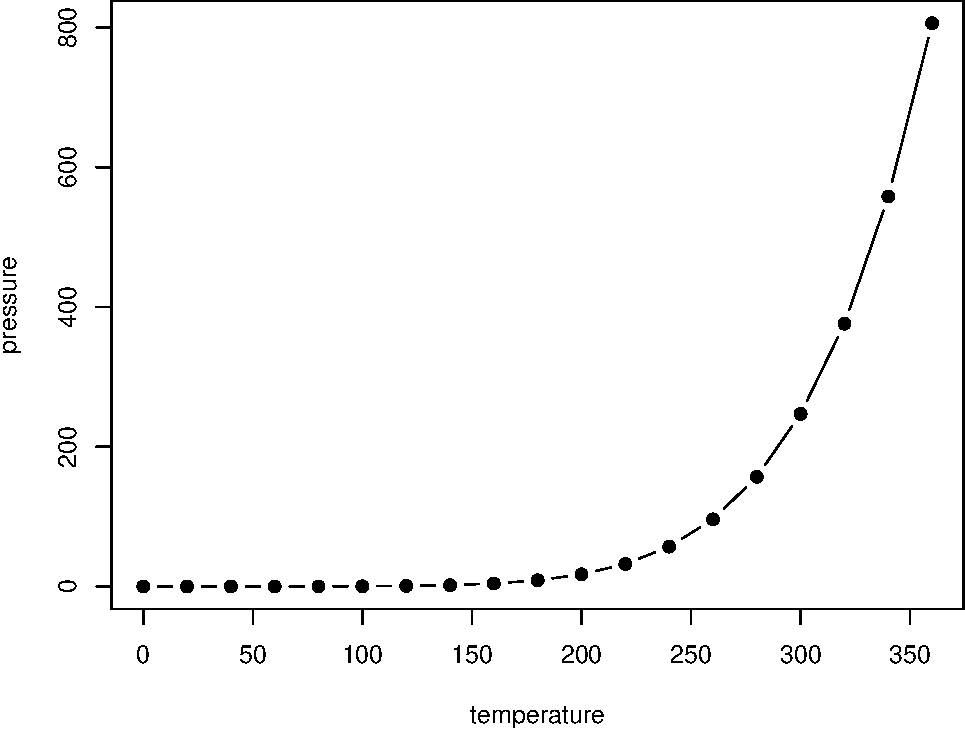
\includegraphics[width=0.8\linewidth]{t02-cross-refs_files/figure-latex/nice-fig-1} 

}

\caption{Here is a nice figure!}\label{fig:nice-fig}
\end{figure}

Don't miss Table \ref{tab:nice-tab}.

\begin{Shaded}
\begin{Highlighting}[]
\NormalTok{knitr}\SpecialCharTok{::}\FunctionTok{kable}\NormalTok{(}
  \FunctionTok{head}\NormalTok{(pressure, }\DecValTok{10}\NormalTok{), }\AttributeTok{caption =} \StringTok{\textquotesingle{}Here is a nice table!\textquotesingle{}}\NormalTok{,}
  \AttributeTok{booktabs =} \ConstantTok{TRUE}
\NormalTok{)}
\end{Highlighting}
\end{Shaded}

\begin{table}

\caption{\label{tab:nice-tab}Here is a nice table!}
\centering
\begin{tabular}[t]{rr}
\toprule
temperature & pressure\\
\midrule
0 & 0.0002\\
20 & 0.0012\\
40 & 0.0060\\
60 & 0.0300\\
80 & 0.0900\\
\addlinespace
100 & 0.2700\\
120 & 0.7500\\
140 & 1.8500\\
160 & 4.2000\\
180 & 8.8000\\
\bottomrule
\end{tabular}
\end{table}

\hypertarget{parts}{%
\chapter{Parts}\label{parts}}

You can add parts to organize one or more book chapters together. Parts can be inserted at the top of an .Rmd file, before the first-level chapter heading in that same file.

Add a numbered part: \texttt{\#\ (PART)\ Act\ one\ \{-\}} (followed by \texttt{\#\ A\ chapter})

Add an unnumbered part: \texttt{\#\ (PART\textbackslash{}*)\ Act\ one\ \{-\}} (followed by \texttt{\#\ A\ chapter})

Add an appendix as a special kind of un-numbered part: \texttt{\#\ (APPENDIX)\ Other\ stuff\ \{-\}} (followed by \texttt{\#\ A\ chapter}). Chapters in an appendix are prepended with letters instead of numbers.

\hypertarget{footnotes-and-citations}{%
\chapter{Footnotes and citations}\label{footnotes-and-citations}}

\hypertarget{footnotes}{%
\section{Footnotes}\label{footnotes}}

Footnotes are put inside the square brackets after a caret \texttt{\^{}{[}{]}}. Like this one \footnote{This is a footnote.}.

\hypertarget{citations}{%
\section{Citations}\label{citations}}

Reference items in your bibliography file(s) using \texttt{@key}.

For example, we are using the \textbf{bookdown} package \citep{R-bookdown} (check out the last code chunk in index.Rmd to see how this citation key was added) in this sample book, which was built on top of R Markdown and \textbf{knitr} \citep{xie2015} (this citation was added manually in an external file book.bib).
Note that the \texttt{.bib} files need to be listed in the index.Rmd with the YAML \texttt{bibliography} key.

The \texttt{bs4\_book} theme makes footnotes appear inline when you click on them. In this example book, we added \texttt{csl:\ chicago-fullnote-bibliography.csl} to the \texttt{index.Rmd} YAML, and include the \texttt{.csl} file. To download a new style, we recommend: \url{https://www.zotero.org/styles/}

The RStudio Visual Markdown Editor can also make it easier to insert citations: \url{https://rstudio.github.io/visual-markdown-editing/\#/citations}

\hypertarget{blocks}{%
\chapter{Blocks}\label{blocks}}

\hypertarget{equations}{%
\section{Equations}\label{equations}}

Here is an equation.

\begin{equation} 
  f\left(k\right) = \binom{n}{k} p^k\left(1-p\right)^{n-k}
  \label{eq:binom}
\end{equation}

You may refer to using \texttt{\textbackslash{}@ref(eq:binom)}, like see Equation \eqref{eq:binom}.

\hypertarget{theorems-and-proofs}{%
\section{Theorems and proofs}\label{theorems-and-proofs}}

Labeled theorems can be referenced in text using \texttt{\textbackslash{}@ref(thm:tri)}, for example, check out this smart theorem \ref{thm:tri}.

\begin{theorem}
\protect\hypertarget{thm:tri}{}\label{thm:tri}For a right triangle, if \(c\) denotes the \emph{length} of the hypotenuse
and \(a\) and \(b\) denote the lengths of the \textbf{other} two sides, we have
\[a^2 + b^2 = c^2\]
\end{theorem}

Read more here \url{https://bookdown.org/yihui/bookdown/markdown-extensions-by-bookdown.html}.

\hypertarget{callout-blocks}{%
\section{Callout blocks}\label{callout-blocks}}

The \texttt{bs4\_book} theme also includes special callout blocks, like this \texttt{.rmdnote}.

You can use \textbf{markdown} inside a block.

\begin{Shaded}
\begin{Highlighting}[]
\FunctionTok{head}\NormalTok{(beaver1, }\AttributeTok{n =} \DecValTok{5}\NormalTok{)}
\CommentTok{\#\textgreater{}   day time  temp activ}
\CommentTok{\#\textgreater{} 1 346  840 36.33     0}
\CommentTok{\#\textgreater{} 2 346  850 36.34     0}
\CommentTok{\#\textgreater{} 3 346  900 36.35     0}
\CommentTok{\#\textgreater{} 4 346  910 36.42     0}
\CommentTok{\#\textgreater{} 5 346  920 36.55     0}
\end{Highlighting}
\end{Shaded}

It is up to the user to define the appearance of these blocks for LaTeX output.

You may also use: \texttt{.rmdcaution}, \texttt{.rmdimportant}, \texttt{.rmdtip}, or \texttt{.rmdwarning} as the block name.

The R Markdown Cookbook provides more help on how to use custom blocks to design your own callouts: \url{https://bookdown.org/yihui/rmarkdown-cookbook/custom-blocks.html}

\hypertarget{sharing-your-book}{%
\chapter{Sharing your book}\label{sharing-your-book}}

\hypertarget{publishing}{%
\section{Publishing}\label{publishing}}

HTML books can be published online, see: \url{https://bookdown.org/yihui/bookdown/publishing.html}

\hypertarget{pages}{%
\section{404 pages}\label{pages}}

By default, users will be directed to a 404 page if they try to access a webpage that cannot be found. If you'd like to customize your 404 page instead of using the default, you may add either a \texttt{\_404.Rmd} or \texttt{\_404.md} file to your project root and use code and/or Markdown syntax.

\hypertarget{metadata-for-sharing}{%
\section{Metadata for sharing}\label{metadata-for-sharing}}

Bookdown HTML books will provide HTML metadata for social sharing on platforms like Twitter, Facebook, and LinkedIn, using information you provide in the \texttt{index.Rmd} YAML. To setup, set the \texttt{url} for your book and the path to your \texttt{cover-image} file. Your book's \texttt{title} and \texttt{description} are also used.

This \texttt{bs4\_book} provides enhanced metadata for social sharing, so that each chapter shared will have a unique description, auto-generated based on the content.

Specify your book's source repository on GitHub as the \texttt{repo} in the \texttt{\_output.yml} file, which allows users to view each chapter's source file or suggest an edit. Read more about the features of this output format here:

\url{https://pkgs.rstudio.com/bookdown/reference/bs4_book.html}

Or use:

\begin{Shaded}
\begin{Highlighting}[]
\NormalTok{?bookdown}\SpecialCharTok{::}\NormalTok{bs4\_book}
\end{Highlighting}
\end{Shaded}


  \bibliography{book.bib,packages.bib}

\end{document}
